%%%%%%%%%%%%%%%%%%%%%%%%%%%%%%%%%%%%
%                                  %
% Titre  : m.tex                   %
% Sujet  : Maintenance manual      %
%          Document body           %
% Auteur : Francois Pellegrini     %
%                                  %
%%%%%%%%%%%%%%%%%%%%%%%%%%%%%%%%%%%%

%% Formatage et pagination.

\documentclass{article}
\usepackage{a4}
\usepackage{courier}
\usepackage{fancyvrb}
\usepackage{url}
\usepackage{hyperref}
\usepackage{breakurl}
\hypersetup{pdfborder={0 0 0},colorlinks=false}
\usepackage[dvips]{graphicx}
\usepackage{xspace}

\usepackage{listings}
% http://mirrors.fe.up.pt/pub/CTAN/macros/latex/contrib/listings/listings.pdf
\lstset{
  basicstyle=\footnotesize\ttfamily,
  frame=single,
  numbers=left,
  numberstyle=\tiny,
  stepnumber=1,
  columns=fullflexible,
  showstringspaces=false,
% tabsize=1,
  breaklines=true,
  breakatwhitespace=false,
}
\lstdefinestyle{language-b}
{
  language=bash,
}
\lstdefinestyle{language-c}
{
  language=C,
}
\lstdefinestyle{language-f}
{
  language=Fortran,
}

\sloppy                                          % Get rid of overfull hbox'es
\renewcommand{\baselinestretch}{1.05}            % Height of linex x 1.05

\setcounter{secnumdepth}{3}                      % Numbered sub-subsections
\setcounter{tocdepth}{3}                         % Sub-subsections in table of contents

%% Macros and useful commands.

\makeatletter
\@definecounter{enumv}                           % 8 levels of itemization
\@definecounter{enumvi}
\@definecounter{enumvii}
\@definecounter{enumviii}
\def\itemize{\ifnum \@itemdepth >8 \@toodeep\else \advance\@itemdepth \@ne
\edef\@itemitem{labelitem\romannumeral\the\@itemdepth}%
\list{\csname\@itemitem\endcsname}{\def\makelabel##1{\hss\llap{##1}}}\fi}
\let\enditemize =\endlist

\def\@iteme[#1]{\if@noparitem \@donoparitem      % Item long pour options
  \else \if@inlabel \indent \par \fi
         \ifhmode \unskip\unskip \par \fi
         \if@newlist \if@nobreak \@nbitem \else
                        \addpenalty\@beginparpenalty
                        \addvspace\@topsep \addvspace{-\parskip}\fi
           \else \addpenalty\@itempenalty \addvspace\itemsep
          \fi
    \global\@inlabeltrue
\fi
\everypar{\global\@minipagefalse\global\@newlistfalse
          \if@inlabel\global\@inlabelfalse
             \setbox\@tempboxa\hbox{#1}\relax
             \hskip \itemindent \hskip -\parindent
             \hskip -\labelwidth \hskip -\labelsep
             \ifdim \wd\@tempboxa > \labelwidth
               \box\@tempboxa\hfil\break
             \else
               \hbox to\labelwidth{\box\@tempboxa\hfil}\relax
               \hskip \labelsep
             \fi
             \penalty\z@ \fi
          \everypar{}}\global\@nobreakfalse
\if@noitemarg \@noitemargfalse \if@nmbrlist \refstepcounter{\@listctr}\fi \fi
\ignorespaces}
\def\iteme{\@ifnextchar [{\@iteme}{\@noitemargtrue \@iteme[\@itemlabel]}}

\let\@Hxfloat\@xfloat
\def\@xfloat#1[{\@ifnextchar{H}{\@HHfloat{#1}[}{\@Hxfloat{#1}[}}
\def\@HHfloat#1[H]{%
\expandafter\let\csname end#1\endcsname\end@Hfloat
\vskip\intextsep\def\@captype{#1}\parindent\z@
\ignorespaces}
\def\end@Hfloat{\vskip \intextsep}
\makeatother

\newcommand{\bn}{\begin{displaymath}}            % Equations non-numerotees
\newcommand{\en}{\end{displaymath}}
\newcommand{\bq}{\begin{equation}}               % Equations numerotees
\newcommand{\eq}{\end{equation}}

\newcommand{\lbo}{\linebreak[0]}
\newcommand{\lbt}{\linebreak[2]}
\newcommand{\noi}{{\noindent}}                   % No indentation
\newcommand{\spa}{{\protect \vspace{\bigskipamount}}} % Vertical spacing

\newcommand{\eg}{{e\@.g\@.}\xspace}              % e.g.
\newcommand{\ie}{\textit{i\@.e\@.}\xspace}       % i.e.

\newcommand{\scotch}{\textsc{Scotch}\xspace}     % "scotch"
\newcommand{\libscotch}{\textsc{libScotch}\xspace} % "libscotch"
\newcommand{\ptscotch}{\textsc{PT-Scotch}\xspace} % "PT-Scotch"
\newcommand{\libptscotch}{\textsc{libPTScotch}\xspace} % "libPTScotch"
\newcommand{\esmumps}{\textsc{esMUMPS}\xspace}   % "esMUMPS"

\newcommand{\UB}{{\rm UB}}                       % UB

%% Version du document.

%%%%%%%%%%%%%%%%%%%%%%%%%%%%%%%%%%%%
%                                  %
% Title    : version.tex           %
% Function : Version labels for    %
%            all documentation     %
% Author   : Francois Pellegrini   %
%                                  %
%%%%%%%%%%%%%%%%%%%%%%%%%%%%%%%%%%%%

\newcommand{\scotchver}{7.0}
\newcommand{\scotchversub}{7.0.5}


%% Page de garde.

\begin{document}

\date{\today}

\title{
\includegraphics{../misc/scotch_logo_color.ps}\\[1em]
       {\LARGE\bf \scotch\ \textsc{\scotchver} Maintainer's Guide}\\[1em]%
       {\normalsize (version \scotchversub)}
}

\author{Fran\c cois Pellegrini\\
Universit\'e de Bordeaux \& LaBRI, UMR CNRS 5800\\
TadAAM team, INRIA Bordeaux Sud-Ouest\\
351 cours de la Lib\'eration, 33405 TALENCE, FRANCE\\
{\tt francois.pellegrini@u-bordeaux.fr}}

\maketitle

\begin{abstract}
This document describes some internals of the \libscotch\
library.
\end{abstract}

\clearpage

\tableofcontents

%%%%%%%%%%%%%%%%%%%%%%%%%%%%%%%%%%%%
%                                  %
% Titre  : s_i.tex                 %
% Sujet  : Manuel de maintenance   %
%          du projet 'Scotch'      %
%          Introduction            %
% Auteur : Francois Pellegrini     %
%                                  %
%%%%%%%%%%%%%%%%%%%%%%%%%%%%%%%%%%%%

\section{Introduction}

This document is a starting point for the persons interested in using
\scotch\ as a testbed for their new partitioning methods, and/or
willing to contribute to it by making these methods available to the
rest of the scientific community.

Much information is missing. If you need specific information, please
send an e-mail, so that relevant additional information can be added
to this document.
                                  % Introduction
%%%%%%%%%%%%%%%%%%%%%%%%%%%%%%%%%%%%
%                                  %
% Titre  : m_n.tex                 %
% Sujet  : Maintenance manual of   %
%          Scotch                  %
%          Style and naming        %
%          conventions             %
% Auteur : Francois Pellegrini     %
%                                  %
%%%%%%%%%%%%%%%%%%%%%%%%%%%%%%%%%%%%

\section{Coding style}

The \scotch\ coding style is now well established. Hence, potential
contributors are requested to abide by it, to provide a global ease of
reading while browsing the code, and to ease the work of their
followers.

In this section, the numbering of the characters of each line is
assumed to start from zero.

\subsection{Typing}

\subsubsection{Spacing}

Expressions are like sentences, where words are separated by
spaces. Hence, an expression like ``\texttt{if~(n == NULL)~\{}''
reads: ``if $n$ is-equal-to NULL then'', with words separated by
single spaces.

As in standard typesetting, there is no space after an opening
parenthesis, nor before a closing one, because they are not words.

When it follows a keyword, an opening brace is always on the same line
as the keyword (save for special cases, e.g. preprocessing macros
between the keyword and the opening brace). This is meant to maximize
the number of ``useful readable lines'' on the screen. However,
closing braces are on a separate line, aligned with the indent of the
line that contains the matching opening brace. This is meant to find
in a glance the line that contains this opening brace.

Brackets are not considered as words: they are stuck both to the word
on their left and the word on their right.

Reference and dereference operators ``\texttt{\&}'' and ``\texttt{*}''
are stuck to the word on their right. However, the multiplication
operator ``\texttt{*}'' counts as a word in arithmetic expressions.

Semicolons are always stuck to the word on their left, except when
they follow an empty instruction, e.g., an empty loop body or an empty
\texttt{for} field. Empty instructions are materialized by a single
space character, which makes the semicolon separated from the
preceding word. For instance: ``\texttt{for~(~;~;~)~;}''.

Ternary operator elements ``\texttt{?}'' and ``\texttt{:}'' are
considered as words and are surrounded by spaces. When the ternary
construct spans across multiple lines, they are placed at the
beginning of each line, before the expression they condition, and not
at the end of the previous line.

\subsubsection{Aligning}

When several consecutive lines contain similar expressions that are
strongly connected, e.g. arguments of a \texttt{mem\lbt Alloc\lbt
  Group()} routine, or assignments of multiple fields of the same
structure(s), extra spaces can be added to align parts of the
expressions. This is a matter of style and opportunity.

For instance, when consecutive lines contain function calls where
opening parentheses are close to each other and their arguments
overlap, open parentheses have to be aligned. However, when arguments
do not overlap, alignment is not required (e.g., for \texttt{return}
statements with small parameters).

\subsubsection{Idiomatic specificities}

While, in C, \texttt{return} is a keyword which does not need
parentheses around its argument, the \scotch\ coding style treats it
as if it were a function call, thus requiring parentheses around its
argument when it has one.

\subsection{Indenting}

Indenting is subject to the following rules:
\begin{itemize}
\item
  All indents are of two characters. Hence, starting from column zero,
  all lines start at even column numbers.
\item
  Tabs are never used in the source code. If your text editor replaces
  chunks of spaces by tabs, it is your duty to disable this feature or
  to make sure to replace all tabs by spaces before the files are
  committed. Unwanted tabs are shown in red when performing a
  ``\texttt{git diff}'' prior to committing.
\end{itemize}

Condition bodies are always indented on the line below the condition
statement. ``\texttt{if}'' statements are always placed at the beginning
of a new line, except when used as an ``\texttt{else~if}''
construct, in which the two keywords appear on the same line,
separated by a single space.

Loop bodies are always indented on the line below the loop statement,
except when the loop body is an empty instruction. In this case, the
terminating semicolon is placed on the same line as the loop
statement, after a single space.

\subsection{Comments}

All comments are C-style, that is, of the form
``\texttt{/*}$\ldots$\texttt{*/}''. C++-style comments should never be
used.

There are three categories of comments: file comments, function/data
structure comments, and line comments. Commenting is subject to the
following rules:
\begin{itemize}
\item
  File comments are standard header blocks that must be copied as
  is. Hence, there is little to say about them. On top of each file
  should be placed a license header, which depends on the origin of
  the file.
\item
  Block comments start with ``\texttt{/*}'' and end with
  ``\texttt{*/}'' on a separate subsequent line. Intermediate lines
  start with ``\texttt{**}''. All these comment markers are placed at
  colums zero. Comment text is separated from the comment markers by a
  single space character. Text in block comments is made of titles or
  of full sentences, that are terminated with a punctuation sign (most
  often a final dot).
\item
  Line comments are of two types: structure definition line comments
  in header files, and code line comments.

  Structure definition line comments in header files start with
  ``\texttt{/*+}'' and end with ``\texttt{+*/}''. This is an old
  Doxygen syntax, which has been preserved over time. Code line
  comments start classically with ``\texttt{/*}'' and end with
  ``\texttt{*/}''.

  All these comments start at least at character~$50$. If the C code
  line is longer, comment lines start one character after the end of
  the line, after a single space. End comment markers are placed at
  least one character after the end of the comment text. When several
  line comments are present on consecutive lines, comment terminators
  are aligned to the farthest comment terminator.

  Comment text always starts with an uppercase letter, and have no
  terminating punctuation sign. They are written in the imperative
  mode, and a positive form (no question asked).

  Line comments for C pre-processing conditional macros
  (e.g. ``\texttt{\#else}'' or ``\texttt{\#endif}'') are not subject
  to indentation rules. They start one character after the keyword,
  and are not subject to end marker alignment, except when consecutive
  lines bear the same keyword (\textit{i.e.}, a ``\texttt{\#endif}''
  statement).
\end{itemize}

\section{Naming conventions}
\label{sec-naming}

Data types, variables, structure fields and function names follow
strict naming conventions. These conventions strongly facilitate the
understanding of the meaning of the expressions, and prevent from
coding mistakes. For instance, ``\texttt{verttax[edgenum]}'' would
clearly be an invalid expression, as a vertex array cannot be indexed
by an edge number. Hence, potential contributors are required to
follow them strictly.

\subsection{File inclusion markers}
\label{sec-naming-file-inclusion-markers}

File inclusion markers are \texttt{\#define}'s which indicate that a
given source file (either a ``\texttt{.c}'' source code file or a
``\texttt{.h}'' header file) has been already encountered.

To minimize risks of collisions with symbols of external libraries,
file inclusion markers start with a prefix that represents the name of
the project, followed by the name of the file in question (without its
type suffix). While filenames can be long, this is not an issue since
the length of the significant part of C~preprocessor symbols is at
least 63~characters\footnote{See e.g.
\url{https://gcc.gnu.org/onlinedocs/cpp/Implementation-limits.html}},
thus longer than that of C identifiers, which is 32~characters.
Header file marker identifiers are suffixed with ``\texttt{\_H}'',
while C source file markers have no suffix.

In order to further minimize risks of collisions, file inclusion
markers should be placed in a file only when needed, that is, when
effectively used as the parameter of a conditional inclusion statement
within another source file.

The current project prefixes are:
\begin{itemize}
\item
  \texttt{SCOTCH\_}: the \scotch\ project itself;
\item
  \texttt{ESMUMPS\_}: the \esmumps\ library, which is treated as a
  separate project to avoid conflicts with data structures and files
  that exist in both libraries, such as \texttt{Graph}'s.
\end{itemize}

\subsection{Variables and fields}
\label{sec-naming-variables}

Variables and fields of the sequential \scotch\ software are commonly
built from a radical and a suffix. When contextualization is required,
e.g., the same kind of variable appear in two different objects, a
prefix is added. In \ptscotch, a second radical is commonly used, to
inform on variable locality or duplication across processes.

Common radicals are:
\begin{itemize}
\item
\texttt{vert}: vertex.
\item
\texttt{velo}: vertex load.
\item
\texttt{vnum}: vertex number, used as an index to access another vertex
structure. This radical typically relates to an array that contains
the vertex indices, in some original graph, corresponding to the
vertices of a derived graph (e.g., an induced graph).
\item
\texttt{vlbl}: user-defined vertex label (at the user API level).
\item
\texttt{edge}: edge (\texttt{i.e.}, arcs, in fact).
\item
\texttt{edlo}: edge (arc) load.
\item
\texttt{arch}: target architecture.
\item
\texttt{graf}: graph.
\item
\texttt{mesh}: mesh.
\end{itemize}

Common suffices are:
\begin{itemize}
\item
\texttt{bas}: start ``based'' value for a number range; see the
``\texttt{nnd}'' suffix below. For number basing and array indexing,
see Section~\ref{sec-basing}.
\item
\texttt{end}: vertex end index of an edge (e.g.,
\texttt{vertend}, wrt. \texttt{vertnum}). The \texttt{end} suffix is
a sub-category of the \texttt{num} suffix.
\item
\texttt{nbr}: number of instances of objects of a given radical
type (e.g., \texttt{vertnbr}, \texttt{edgenbr}). They are commonly
used within ``un-based'' loop constructs, such as:
``\texttt{for (vertnum = 0; vertnum < vertnbr; vertnum ++)} \ldots''.
\item
\texttt{nnd}: end based value for a number range, commonly used
for loop boundaries. Usually, $\mbox{*\texttt{nnd}} =
\mbox{*\texttt{nbr}} + \mbox{\texttt{baseval}}$. For instance,
$\mbox{\texttt{vertnnd}} = \mbox{\texttt{vertnbr}} +
\mbox{\texttt{baseval}}$. They are commonly used in based loop
constructs, such as:
``\texttt{for (vertnum = baseval; vertnum < vertnnd; vertnum ++)}
\ldots''. For local vertex ranges, e.g., within a thread that manages
only a partial vertex range, the loop construct would be:
``\texttt{for (vertnum = vertbas; vertnum < vertnnd; vertnum ++)}
\ldots''.
\item
\texttt{num}: based or un-based number (index) of some instance of an
object of a given radical type. For instance, \texttt{vertnum} is the
index of some (graph) vertex, that can be used to access adjacency
(\texttt{verttab}) or vertex load (\texttt{velotab}) arrays.
$0 \leq \mbox{\texttt{vertnum}} < \mbox{\texttt{vertnbr}}$ if the
vertex index is un-based, and $\mbox{\texttt{baseval}} \leq
\mbox{\texttt{vertnum}} < \mbox{\texttt{vertnnd}}$
if the index is based, that it, counted starting from
\texttt{baseval}.
\item
\texttt{ptr}: pointer to an instance of an item of some radical type
(e.g., \texttt{grafptr}).
\item
\texttt{sum}: sum of several values of the same radical type (e.g.,
\texttt{velosum}, \texttt{edlosum}).
\item
\texttt{tab}: reference to the first memory element of an array. Such
a reference is returned by a memory allocation routine (e.g.,
\texttt{mem\lbt Alloc}) or allocated from the stack.
\item
\texttt{tax} (for ``\textit{table access}''): reference to an array
that will be accessed using based indices. See
Section~\ref{sec-basing}.
\item
\texttt{tnd}: pointer to the based after-end of an array of items
of radix type (e.g. \texttt{velotnd}). Variables of this suffix are
mostly used as bounds in loops.
\item
\texttt{val}: value of an item. For instance, \texttt{baseval} is the
indexing base value, and \texttt{veloval} is the load of some vertex,
that may have been read from a file.
\end{itemize}

Common prefixes are:
\begin{itemize}
\item
\texttt{src}: source, wrt. active. For instance, a source graph is a
plain \texttt{Graph} structure that contains only graph topology,
compared to enriched graph data structures that are used for specific
computations such as bipartitioning.
\item
\texttt{act}: active, wrt. source. An active graph is a data structure
enriched with information required for specific computations, e.g. a
\texttt{Bgraph}, a \texttt{Kgraph} or a \texttt{Vgraph} compared to a
\texttt{Graph}.
\item
\texttt{ind}: induced, wrt. original.
\item
\texttt{src}: source, wrt. active or target.
\item
\texttt{org}: original, wrt. induced. An original graph is a graph
from which a derived graph will be computed, e.g. an induced subgraph.
\item
\texttt{tgt}: target.
\item
\texttt{coar}: coarse, wrt. fine (e.g. \texttt{coarvertnum}, as a
variable that holds the number of a coarse vertex, within some
coarsening algorithm).
\item
\texttt{fine}: fine, wrt. coarse.
\item
\texttt{mult}: multinode, for coarsening.
\end{itemize}

\subsection{Functions}
\label{sec-naming-functions}

Like variables, routines of the \scotch\ software package follow a
strict naming scheme, in an object-oriented fashion. Routines are
always prefixed by the name of the data structure on which they
operate, then by the name of the method that is applied to the said
data structure. Some method names are standard for each class.

Standard method names are:
\begin{itemize}
\item
\texttt{Alloc}: dynamically allocate an object of the given class. Not
always available, as many objects are allocated on the stack as local
variables.
\item
\texttt{Init}: initialization of the object passed as parameter.
\item
\texttt{Free}: freeing of the external structures of the object, to save
space. The object may still be used, but it is considered as ``empty''
(e.g., an empty graph). The object may be re-used after it is
initialized again.
\item
\texttt{Exit}: freeing of the internal structures of the object. The
object must not be passed to other routines after the \texttt{Exit}
method has been called.
\item
\texttt{Copy}: make a fully operational, independent, copy of the
object, like a ``clone'' function in object-oriented languages.
\item
\texttt{Load}: load object data from stream.
\item
\texttt{Save}: save object data to stream.
\item
\texttt{View}: display internal structures and statistics, for debugging
purposes.
\item
\texttt{Check}: check internal consistency of the object data, for
debugging purposes. A \texttt{Check} method must be created for any
new class, and any function that creates or updates an instance of
some class must call the appropriate \texttt{Check} method, when
compiled in debug mode.
\end{itemize}

\subsection{Array index basing}
\label{sec-basing}

The \libscotch\ library can accept data structures that come both from
FORTRAN, where array indices start at $1$, and C, where they start at
$0$. The start index for arrays is called the ``base value'', commonly
stored in a variable (or field) called \texttt{baseval}.

In order to manage based indices elegantly, most references to arrays
are based as well. The ``table access'' reference, suffixed as
``\texttt{tax}'' (see Section~\ref{sec-naming-variables}), is defined
as the reference to the beginning of an array in memory, minus the
base value (with respect to pointer arithmetic, that is, in terms of
bytes, times the size of the array cell data type). Consequently, for
any array whose beginning is pointed to by \texttt{xxxxtab}, we have
$\mbox{\texttt{xxxxtax}} = \mbox{\texttt{xxxxtab}} - \mbox{\texttt{baseval}}$.
Consequently \texttt{xxxxtax[baseval]} always represents the first
cell in the array, whatever the base value is.
Of course, memory allocation and freeing operations must always
operate on \texttt{tab} pointers only.

In terms of indices, if the size of the array is \texttt{xxxxnbr},
then
$\mbox{\texttt{xxxxnnd}} = \mbox{\texttt{xxxxnbr}} + \mbox{\texttt{baseval}}$,
so that valid indices \texttt{xxxxnum} always belong to the range
$[\mbox{\texttt{baseval}};\mbox{\texttt{vertnnd}}[$. Consequently,
loops often take the form:
\begin{center}
{\renewcommand{\baselinestretch}{1.05}
\footnotesize\tt
\begin{verbatim}
  for (xxxxnum = baseval; xxxxnum < xxxxnnd; xxxxnum ++) {
    xxxxtax[xxxxnum] = ...;
  }
\end{verbatim}
}
\end{center}
                                  % Naming conventions
%%%%%%%%%%%%%%%%%%%%%%%%%%%%%%%%%%%%
%                                  %
% Title   : m_s.tex                %
% Subject : Maintenance manual of  %
%           Scotch                 %
%           Global structure       %
% Author  : Francois Pellegrini    %
%                                  %
%%%%%%%%%%%%%%%%%%%%%%%%%%%%%%%%%%%%

\section{Structure of the \libscotch\ library}
\label{sec-structure}

As seen in Section~\ref{sec-naming-functions}, all of the routines
that comprise the \libscotch\ project are named with a prefix that
defines the type of data structure onto which they apply and a prefix
that describes their purpose. This naming scheme allows one to
categorize functions as methods of classes, in an object-oriented
manner.

This organization is reflected in the naming and contents of the
various source files.

The main modules of the \libscotch\ library are the following:
\begin{itemize}
\item
\texttt{arch}: target architectures used by the static mapping methods.
\item
\texttt{bgraph}: graph edge bipartitioning methods, hence the initial.
\item
\texttt{graph}: basic (source) graph handling methods.
\item
\texttt{hgraph}: graph ordering methods. These are based on an extended
``halo'' graph structure, thus for the initial.
\item
\texttt{hmesh}: mesh ordering methods.
\item
\texttt{kgraph}: k-way graph partitioning methods.
\item
\texttt{library}: API routines for the \libscotch\ library.
\item
\texttt{mapping}: definition of the mapping structure.
\item
\texttt{mesh}: basic mesh handling methods.
\item
\texttt{order}: definition of the ordering structure.
\item
\texttt{parser}: strategy parsing routines, based on the \textsc{Flex}
and \textsc{Bison} parsers.
\item
\texttt{vgraph}: graph vertex bipartitioning methods, hence the initial.
\item
\texttt{vmesh}: mesh node bipartitioning methods.
\end{itemize}

Every source file name is made of the name of the module to which it
belongs, followed by one or two words, separated by an underscore,
that describe the type of action performed by the routines of the
file. For instance, for module \texttt{bgraph}:
\begin{itemize}
\item
\texttt{bgraph.h} is the header file that defines the \texttt{Bgraph}
data structure,
\item
\texttt{bgraph\_bipart\_fm.[ch]} are the files that contain the
Fiduccia-Mattheyses-like graph bipartitioning method,
\item
\texttt{bgraph\_check.c} is the file that contains the consistency
checking routine \texttt{bgraph\lbt Check} for \texttt{Bgraph}
structures,
\end{itemize}
and so on. Every source file has a comments header briefly describing
the purpose of the code it contains.
                                  % Structure of the libScotch
%%%%%%%%%%%%%%%%%%%%%%%%%%%%%%%%%%%%
%                                  %
% Titre  : m_f.tex                 %
% Sujet  : Maintenance manual of   %
%          Scotch                  %
%          File formats v6.0       %
% Auteur : Francois Pellegrini     %
%                                  %
%%%%%%%%%%%%%%%%%%%%%%%%%%%%%%%%%%%%

\section{Files and data structures}
\label{sec-file}

User-manageable file formats are described in the \scotch user's
guide. This section contains information that are relevant only to
developers and maintainers.

For the sake of portability, readability, and reduction of storage space,
all the data files shared by the different programs of the
\scotch\ project are coded in plain ASCII text exclusively.
Although one may speak of ``lines'' when describing file formats,
text-formatting characters such as newlines or tabulations are not
mandatory, and are not taken into account when files are read.
They are only used to provide better readability and understanding.
Whenever numbers are used to label objects, and unless explicitely
stated, \textbf{numberings always start from zero}, not one.

\subsection{Decomposition-defined architecture files}
\label{sec-file-target-deco-one}

Decomposition-defined architecture files are the way to describe
irregular target architectures that cannot be represented as
algorithmically-coded architectures.

Two main file formats coexist: the ``\texttt{deco 0}'' and
``\texttt{deco 2}'' formats. ``\texttt{deco}'' stands for
``decomposition-defined architecture'', followed by the format
number. The ``\texttt{deco 1}'' format is a compiled form of the
``\texttt{deco 0}'' format. We will describe it here.

The ``\texttt{deco 1}'' file format results from an $O(p^2)$
preprocessing of the ``\texttt{deco 0}'' target architecture
format. While the ``\texttt{deco 0}'' format contains a distance
matrix between all pairs of terminal domains, which is consequently in
in $\Theta(p^2/2)$, the ``\texttt{deco 1}'' format contains the
distance matrix between any pair of domains, whether they are terminal
or not. Since there are roughly $2p$ non-terminal domains in a
target architecture with $p$ terminal domains, because all domains
form a binary tree whose leaves are the terminal domains, the distance
matrix of a ``\texttt{deco 1}'' format is in $\Theta(2p^2)$, that is,
four times that of the corresponding ``\texttt{deco 0}'' file.

Also, while the ``\texttt{deco 0}'' format lists only the
characteristics of terminal domains (in terms of weights and labels),
the ``\texttt{deco 1}'' format provides these for all domains, so as
to speed-up the retrieval of the size, weight and label of any domain,
whether it is terminal or not.

The ``\texttt{deco 1}'' header is followed by two integer numbers,
which are the number of processors and the largest terminal number used
in the decomposition, respectively (just as for ``\texttt{deco 0}''
files). Two arrays follow.

The first array has as many lines as there are domains (and not only
terminal domains as in the case of ``\texttt{deco 0}'' files). Each of
these lines holds three numbers: the label of the terminal domain that
is associated with this domain (which is the label of the terminal
domain of smallest number contained in this domain), the size of the
domain, and the weight of the domain.
The first domain in the array is the initial domain holding all the
processors, that is, domain $1$. The other domains in the array are
the resulting subdomains, in ascending domain number order, such that
the two subdomains of a given domain of number $i$ are numbered $2i$
and $2i+1$.

The second array is a lower triangular diagonal-less matrix that gives the
distance between all pairs of domains.

For instance, Figure~\ref{fig-file-targetdeco-zero} and
Figure~\ref{fig-file-targetdeco-one} show the contents of the
``\texttt{deco 0}'' and ``\texttt{deco 1}'' architecture decomposition
files for $\UB(2,3)$, the binary de~Bruijn graph of dimension~$3$, as
computed by the \texttt{amk\_grf} program.
\begin{figure}[hbt]
\begin{tabular}{p{0.69\linewidth}@{}p{0.29\linewidth}}
\begin{center}
\parbox[t]{0.9\linewidth}{\vspace{0pt}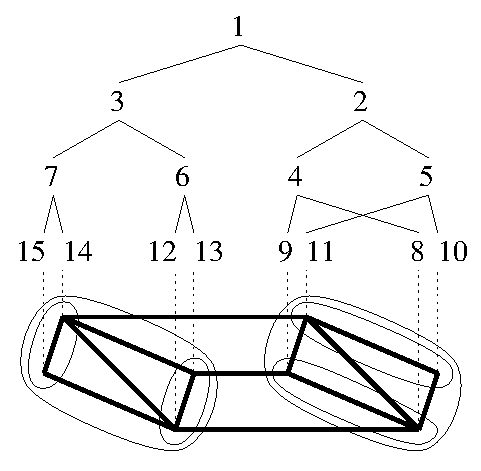
\includegraphics[width=0.7\linewidth]{s_f_d.ps}}
\end{center}
&
\begin{center}
{\renewcommand{\baselinestretch}{1.05}
\footnotesize\tt
\begin{verbatim}
deco 0
8	15
0	1	15
1	1	14
2	1	13
3	1	11
4	1	12
5	1	9
6	1	8
7	1	10
1
2 1
2 1 2
1 1 1 2
3 2 1 1 2
2 2 2 1 1 1
3 2 3 1 2 2 1
\end{verbatim}
}
\end{center}
\end{tabular}
\caption{``\texttt{deco 0}'' target decomposition file for $\UB(2,3)$.
         The terminal numbers associated with every processor define a unique
         recursive bipartitioning of the target graph.}
\label{fig-file-targetdeco-zero}
\end{figure}

\begin{figure}[hbt]
\begin{tabular}{p{0.49\linewidth}@{}p{0.49\linewidth}}
\begin{center}
{\renewcommand{\baselinestretch}{1.05}
\footnotesize\tt
\begin{verbatim}
deco
1
8	15
0	8	8
3	4	4
0	4	4
5	2	2
3	2	2
2	2	2
0	2	2
6	1	1
5	1	1
7	1	1
3	1	1
4	1	1
2	1	1
1	1	1
0	1	1
\end{verbatim}
}
\end{center}
&
\begin{center}
{\renewcommand{\baselinestretch}{1.05}
\footnotesize\tt
\begin{verbatim}
2	2	2	2	1	2	2	1
3	1	2	2	1	2	2	2
3	1	2	2	1	2	1	2
1	1	2	2	3	2	3	1
2	2	3	1	3	2	3	2
1	3	3	1	2	2	1	2
1	1	2	2	1	1	1	2
2	1	2	2	1	1	1	2
2	2	3	3	2	2	3	1
2	2	1	3	2	1	2	2
1	2	2	1	1	2	2	2
1	1	1	3	3	2	3	3
2	1	2	3	3	2	1	2
1
\end{verbatim}
}
\end{center}
\end{tabular}
\caption{``\texttt{deco 1}'' target decomposition file for $\UB(2,3)$,
  compiled with the \texttt{acpl} tool from the ``\texttt{deco 0}''
  file displayed in Figure~\ref{fig-file-targetdeco-zero}.}
\label{fig-file-targetdeco-one}
\end{figure}
                                  % File formats
%%%%%%%%%%%%%%%%%%%%%%%%%%%%%%%%%%%%%%%%%%%
%                                         %
% Title   : m_d.tex                       %
% Subject : Maintenance manual of Scotch  %
%           Data structure explanations   %
% Author  : Francois Pellegrini           %
%                                         %
%%%%%%%%%%%%%%%%%%%%%%%%%%%%%%%%%%%%%%%%%%%

\section{Data structure explanations}
\label{sec-data}

This section explains some of the data structures implemented in
\scotch\ and \ptscotch.

\subsection{\texttt{Dorder}}
\label{sec-data-dorder}

Distributed orderings are data structures used in \ptscotch\ to
represent orderings distributed on a set of processing elements. Like
for the centralized ordering of type \texttt{Order} (see
Section~\ref{sec-data-order}), a distributed ordering consists of an
inverse permutation, which provides the old indices of the reordered
vertices, and a column block decomposition of the reordered matrix, to
help perform more efficient block computations at the solve stage. The
column block decomposition is defined as a tree structure, the nodes
of which, of type \texttt{Dorder\lbt Cblk}, represent column blocks
tree nodes containing consecutive, reordered vertices. A tree node may
have children nodes, which represent the decomposition of a column
block into sub-column blocks, \eg, when a subdomain is decomposed into
two separated subdomains and a separator.

Because its column blocks are distributed across multiple processing
elements, the \texttt{Dorder} data type is much more complex than
the \texttt{Order} data type. Hence, it is important to fully
understand the \texttt{Order} data type before delving into the
meanders of the \texttt{Dorder} data type and its ancillary data
types. The main difference between the two is that, since graphs are
distributed across multiple processing elements, column block
information has to be duplicated on all the processing elements
which contain a piece of a given graph. In order to reconciliate this
information, to provide a centralized block column ordering, all
distributed column block tree node structures are identified by a
\texttt{Dorder\lbt Index} data structure.

The distributed column block tree data structure, created by way of
parallel graph separation algorithms, always ends up in leaves, when
nested dissection no longer succeeds or when the distributed subgraphs
are folded onto single processing elements. As soon as the latter
happens, a purely sequential graph ordering process can take place on
each of them. This leads to the creation of a leaf
\texttt{Dorder\lbt Cblk} node, into which the resulting
locally-computed, centralized column block sub-tree is compacted as an
array of \texttt{Dorder\lbt Node} data structures. From the above, at
the time being, the distributed column block tree structure contains
only either nested dissection nodes, of type
\texttt{DORDER\lbt CBLK\lbt NEDI}, and leaf nodes, of type 
\texttt{DORDER\lbt CBLK\lbt LEAF}. In order to facilitate the
integration of centralized column block sub-trees into a global
distributed column block tree, the values of the type flags are the
same for the \texttt{Dorder} and \texttt{Order} data types.

The fields of the \texttt{Dorder} data structure are the following:
\begin{itemize}
\iteme[\texttt{baseval}]
  Base value for the inverse permutation.
\iteme[\texttt{vnodglbnbr}]
  Overall number of node vertices to order across all processing
  elements. For graph orderings, this number is equal to the number of
  non-halo vertices in the initial graph.
\iteme[\texttt{cblklocnbr}]
  Local number of locally-rooted column blocks. This number is the sum
  of the number of centralized column blocks, of type
  \texttt{Dorder\lbt Node}, held by the current processing element,
  plus the number of distributed column block tree nodes, of type
  \texttt{Dorder\lbt Cblk}, the \texttt{proc\lbt loc\lbt num} index of
  which is equal to the rank of the processing element. This allows
  one to count only once each distributed column block tree node, when
  summing the \texttt{cblk\lbt loc\lbt nbr} fields over all
  processing elements.
\iteme[\texttt{linkdat}]
  Start of the doubly-linked list of distributed column block tree
  nodes, of type \texttt{Dorder\lbt Cblk}, on the given processing
  element. This list is circular, to allow for the insertion of new
  nodes at the end of the list in constant time.
\iteme[\texttt{proccomm}]
  MPI communicator for managing the distributed ordering. It should be
  the same as that of the initial distributed graph to be ordered.
\iteme[\texttt{proclocnum}]
  Rank of the given processing element within the communicator.
\iteme[\texttt{mutelocdat}]
  When multi-threading is activated, allows one to create critical
  sections to update the ordering data in a thread-safe manner.
\end{itemize}

\subsubsection{\texttt{DorderIndex}}
\label{sec-data-dorder-index}

Since the ordering data structure is distributed, pointers cannot be
used to refer to parent or children column block tree node data
structures across processing elements. The \texttt{Dorder\lbt Index}
data type defines an identifier for column block tree nodes. These
identifiers are unique, in the sense that, on each processing element,
no two \texttt{Dorder\lbt Cblk} structures will have the same
identifier. However, several \texttt{Dorder\lbt Cblk} structures may
bear the same \texttt{Dorder\lbt Index} values on different processing
elements, in the case when they are siblings which maintain the local
information about the same distributed column block tree node.

The fields of the \texttt{DorderIndex} data type are the following:
\begin{itemize}
\iteme[\texttt{proclocnum}]
  Smallest rank among the processing elements on which a copy of the
  column block tree node resides.
\iteme[\texttt{cblklocnum}]
  Local number of the column block tree node data structure on the
  processing element of aforementioned rank.
\end{itemize}

\subsubsection{\texttt{DorderLink}}
\label{sec-data-dorder-link}

Since distributed column block tree nodes, of type
\texttt{Dorder\lbt Cblk}, are created on the fly on each processing
element, are in small numbers, and are heavy structures, they are not
stored in a single resizable array, but as individual cells which are
allocated when needed. Consequently, these structures have to be
linked together, for proper management.

The \texttt{DorderLink} data type aims at chaining all
\texttt{Dorder\lbt Cblk} structures in a circular, doubly-linked
list. New nodes are inserted at the end of the list, such that a simple
traversal yields nodes in ascending creation order, which is essential
for locally-rooted nodes when gathering them to create a centralized
ordering. The \texttt{Dorder\lbt Link} structure is the first field of
the \texttt{Dorder\lbt Cblk} structure, so that a simple pointer cast
allows one to retrieve the tree node structure from the current link.

The fields of the \texttt{DorderLink} data structure are the following:
\begin{itemize}
\iteme[\texttt{nextptr}]
  Pointer to the next distributed column block tree node created on
  the given processing element.
\iteme[\texttt{prevptr}]
  Pointer to the previous distributed column block tree node created
  on the given processing element.
\end{itemize}

\subsubsection{\texttt{DorderNode}}
\label{sec-data-dorder-node}

The distributed column block tree data structure ends up in leaves,
when either the parallel nested dissection stops, or when distributed
subgraphs are located on single processing elements. In the first
case, the distributed subgraph is centralized, after which, in both
cases, a centralized ordering strategy is applied to the centralized
subgraph, and a centralized block ordering is computed. This
centralized block ordering is represented as an \texttt{Order}
data structure, containing an inverse permutation and a tree of
\texttt{Order\lbt Cblk} nodes. Since the distributed ordering will
eventually have to be centralized, the local, centralized orderings
will have to be compacted and sent to the root processing
element. In order to anticipate this and to save space, once a
centralized ordering is computed on some processing element, the
resulting column block tree is compacted into a single array of
\texttt{Dorder\lbt Node} cells.

The fields of the \texttt{DorderNode} data type are the following:
\begin{itemize}
\iteme[\texttt{fathnum}]
  Un-based index of the father node of the given node in the node
  array, or $-1$ if the given node is a local root and has to be
  connected to the father of the local leaf of the distributed column
  block tree.
\iteme[\texttt{typeval}]
  Type of centralized column block tree node. The admissible values
  are constants of the kind \texttt{ORDERCBLK*}.
\iteme[\texttt{vnodnbr}]
  Number of node vertices in the column block.
\iteme[\texttt{cblknum}]
  Rank of the tree node among the children of its father, starting
  from zero.
\end{itemize}

Like for the \texttt{Dorder\lbt Cblk} data type, there are no
references from a node to its children, but a reference from each node
to its father, with all information needed to rebuild a global
centralized column block tree when all node information is centralized
on a single processing element.

\subsubsection{\texttt{DorderCblk}}
\label{sec-data-dorder-cblk}

The \texttt{DorderCblk} data type represents distributed column block
tree nodes within distributed orderings. A tree node may be a leaf
node, or have children nodes which describe the decomposition of a
column block into sub-column blocks, \eg, when a graph is decomposed
into two separated subgraphs and a separator.

Since, by nature, every distributed column block tree node concerns a
set of vertices distributed across a set of processing elements, each
of the latter holds a copy of the tree node, the identifier of which,
of type \texttt{Dorder\lbt Index}, contains identical information: the
smallest rank among the involved processing elements within the
communicator used to manage the distributed ordering, and an index
incrementally generated on this processing element. Unlike for the
\texttt{Order} data type, there are no pointers from a tree node to
its child nodes; on the opposite, the \texttt{Dorder\lbt Cblk} node
contains a \texttt{Dorder\lbt Index} referring to its father node. The
only information a tree node will hold about its children is their
number.

The fields of the \texttt{DorderCblk} data type are the following:
\begin{itemize}
\iteme[\texttt{linkdat}]
  Doubly-linked list structure to chain together all
  the \texttt{Dorder\lbt Cblk} structures on a given processing
  element.
\iteme[\texttt{ordelocptr}]
  Pointer to the distributed ordering to which the given distributed
  column block tree node belongs.
\iteme[\texttt{typeval}]
  Type of tree node; at the time being, it is either
  \texttt{DORDER\lbt CBLK\lbt NEDI} for a nested dissection node, or
  \texttt{DORDER\lbt CBLK\lbt LEAF} for a leaf node.
\iteme[\texttt{fathnum}]
  Identifier of the father of the given column block tree node. If the
  given tree node is a root, the value of the father index is
  \texttt{\{~0, -1~\}}.
\iteme[\texttt{cblknum}]
  Identifier of the given column block tree node. The process number
  is the smallest rank among all the processing elements sharing node
  vertices, and the local number is provided incrementally on this
  processing element.
\iteme[\texttt{ordeglbval}]
  Un-based global start index of the node vertices in the distributed
  column block tree node.
\iteme[\texttt{vnodglbnbr}]
  Number of node vertices contained in the distributed column block
  tree node, over all the involved processing elements. If the
  column block has sub-column blocks, the sum of all the
  \texttt{vnodglbnbr} values of the sub-column blocks must be equal to
  the \texttt{vnodglbnbr} of the column block.
\iteme[\texttt{cblkfthnum}]
  Index of the given column block tree node among its siblings,
  starting from zero.
\iteme[\texttt{data}]
  Union field holding the information concerning either the leaf node
  or the nested dissection node. This field has two sub-fields:
  \begin{itemize}
  \iteme[\texttt{leaf}]
    Leaf field, which has the following sub-fields:
    \begin{itemize}
    \iteme[\texttt{ordelocval}]
      Un-based start index in the global inverse permutation array for
      the local vertices.
    \iteme[\texttt{vnodlocnbr}]
      Number of node vertices in the given permutation fragment.
    \iteme[\texttt{periloctab}]
      Pointer to the local, un-based, inverse permutation fragment
      array, of size \texttt{vnod\lbt loc\lbt nbr}. The values of the
      \texttt{peri\lbt loc\lbt tab} array are based according to the
      \texttt{baseval} field of the \texttt{Dorder} data type.
    \iteme[\texttt{nodelocnbr}]
      Number of local column block tree nodes associated with the
      permutation fragment.
    \iteme[\texttt{nodeloctab}]
      Pointer to the local, un-based, array of local column block tree
      nodes, of size \texttt{node\lbt loc\lbt nbr}.
    \iteme[\texttt{cblklocnum}]
      Un-based index, in \texttt{node\lbt loc\lbt tab}, of the root
      local column block tree node.
    \end{itemize}
  \iteme[\texttt{nedi}]
    Nested dissection field. This field has a single sub-field:
    \begin{itemize}
    \iteme[\texttt{cblkglbnbr}]
      Number of sub-column blocks within this column block. For nested
      dissection, this number is either $2$ (two separated parts and
      no separator) or $3$ (two separated parts and a separator).
    \end{itemize}
  \end{itemize}
\end{itemize}

\subsection{\texttt{Graph}}
\label{sec-data-graph}

Graphs are the fundamental underlying data structures of all the
algorithms implemented in \scotch. The \texttt{Graph} structure is the
foundational data structure, from which subclasses will be derived,
according to the specific needs of the \scotch\ modules. It is
sometimes referred to as the \textit{source graph} structure, with
respect to the \textit{target architecture} \texttt{Arch} onto which
source graphs are to be mapped.

The \texttt{Graph} structure, being a foundational data structure,
does not possess any variable fields related to actual computations,
\eg, partition state variables or an execution context. Such fields
will be found in \textit{active} graphs, \eg, \texttt{Bgraph},
\texttt{Kgraph}, \texttt{Vgraph}.

A \texttt{Graph} is described by means of adjacency lists. These data
are stored in arrays and scalars of type \texttt{SCOTCH\_Num}, as
shown in Figures~\ref{fig-lib-graf-one}
and~\ref{fig-lib-graf-two}. The \texttt{Graph} fields have the
following meaning:
\begin{itemize}
\iteme[\texttt{baseval}]
Base value for all array indexing.
\iteme[\texttt{vertnbr}]
Number of vertices in graph.
\iteme[\texttt{edgenbr}]
Number of arcs in graph. Since edges are represented by both of their
ends, the number of edge data in the graph is twice the number of
graph edges.
\iteme[\texttt{verttax}]
Based array of start indices in $\mathtt{edgetax}$ of vertex
adjacency sub-arrays.
\iteme[\texttt{vendtax}]
Based array of after-last indices in $\mathtt{edgetax}$ of vertex
adjacency sub-arrays.
For any vertex $i$, with $\mathtt{baseval} \leq i < (\mathtt{vertnbr}
+ \mathtt{baseval})$, $(\mathtt{vendtax[}i\mathtt{]}
-\mathtt{verttax[}i\mathtt{]})$ is the degree of vertex $i$, and the
indices of the neighbors of $i$ are stored in $\mathtt{edgetax}$ from
$\mathtt{edgetax[\lbt verttax[}i\mathtt{]]}$ to $\mathtt{edgetax[\lbt
vendtax[}i\mathtt{]} - 1\mathtt{]}$, inclusive.

When all vertex adjacency lists are stored in order in
$\mathtt{edgetax}$, it is possible to save memory by not allocating
the physical memory for $\mathtt{vendtax}$. In this case, illustrated
in Figure~\ref{fig-lib-graf-one}, $\mathtt{verttax}$ is of size
$\mathtt{vertnbr} + 1$ and $\mathtt{vendtax}$ points to
$\mathtt{verttax} + 1$. This case is referred to as the ``compact edge
array'' case, such that $\mathtt{verttax}$ is sorted in ascending
order, $\mathtt{verttax[\lbt baseval]} = \mathtt{baseval}$ and
$\mathtt{verttax[\lbt baseval} + \mathtt{vertnbr]} =
(\mathtt{baseval} + \mathtt{edgenbr})$.
\iteme[\texttt{velotax}]
Optional based array, of size $\mathtt{vertnbr}$, holding the integer
load associated with every vertex.
\iteme[\texttt{vnumtax}]
When the current graph is a subgraph of some initial graph, this
based array, of size $\mathtt{vertnbr}$, holds the initial vertex
indices of the subgraph vertices. This array is not defined (\ie,
$\mathtt{vnumtax} = \mathtt{NULL}$) when the graph is the initial
graph.
\iteme[\texttt{edgetax}]
Based array, of a size equal at least to
$\left(\max_{i}(\mathtt{vendtax[}i\mathtt{]}) -
\mathtt{baseval}\right)$, holding the adjacency array of every
vertex.
\iteme[\texttt{edlotax}]
Optional based array, of a size equal at least to
$\left(\max_{i}(\mathtt{vendtax[} i \mathtt{]}) -
\mathtt{baseval}\right)$, holding the integer load associated with
every arc. Matching arcs should always have identical loads.
\end{itemize}

\begin{figure}
\centering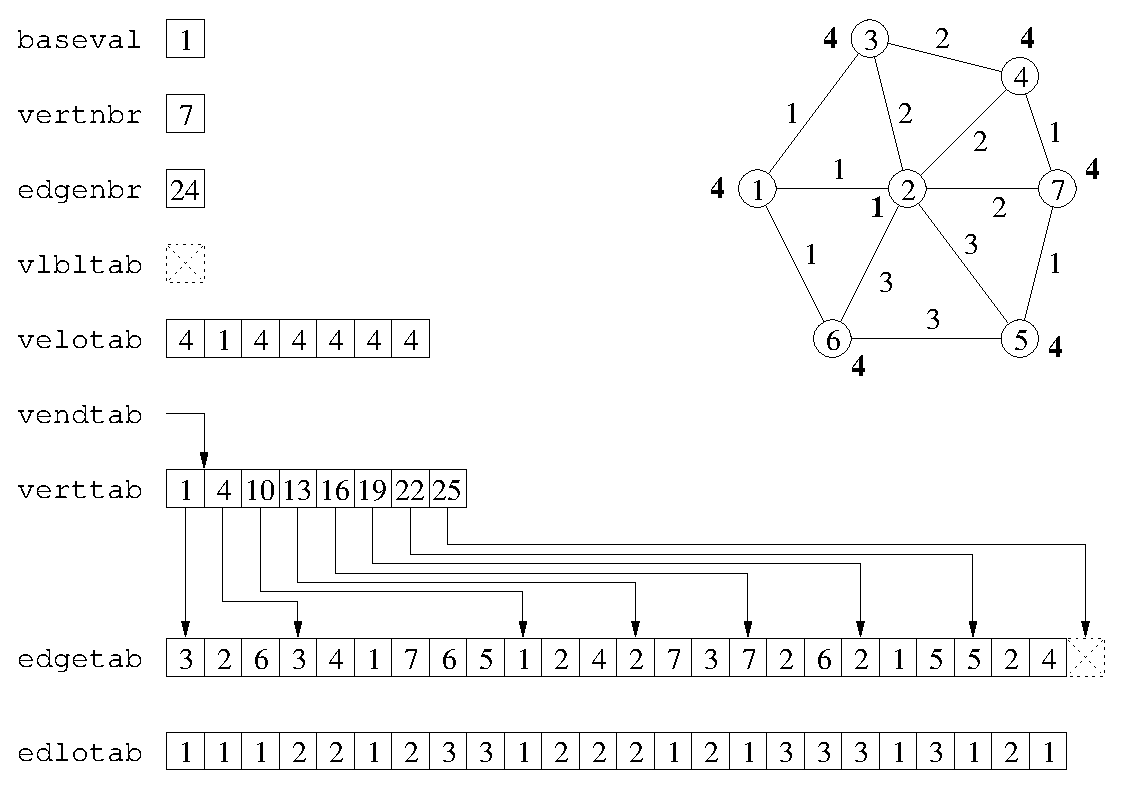
\includegraphics[scale=0.47]{s_f_gr1.eps}
\caption{Sample graph and its description using a compact edge
array. Numbers within vertices are vertex indices, bold numbers
close to vertices are vertex loads, and numbers close to edges are
edge loads. Since the edge array is compact, $\mathtt{verttax}$ is
of size $\mathtt{vertnbr} + 1$ and $\mathtt{vendtax}$ points to
$\mathtt{verttax} + 1$.}
\label{fig-lib-graf-one}
\end{figure}

\begin{figure}
\centering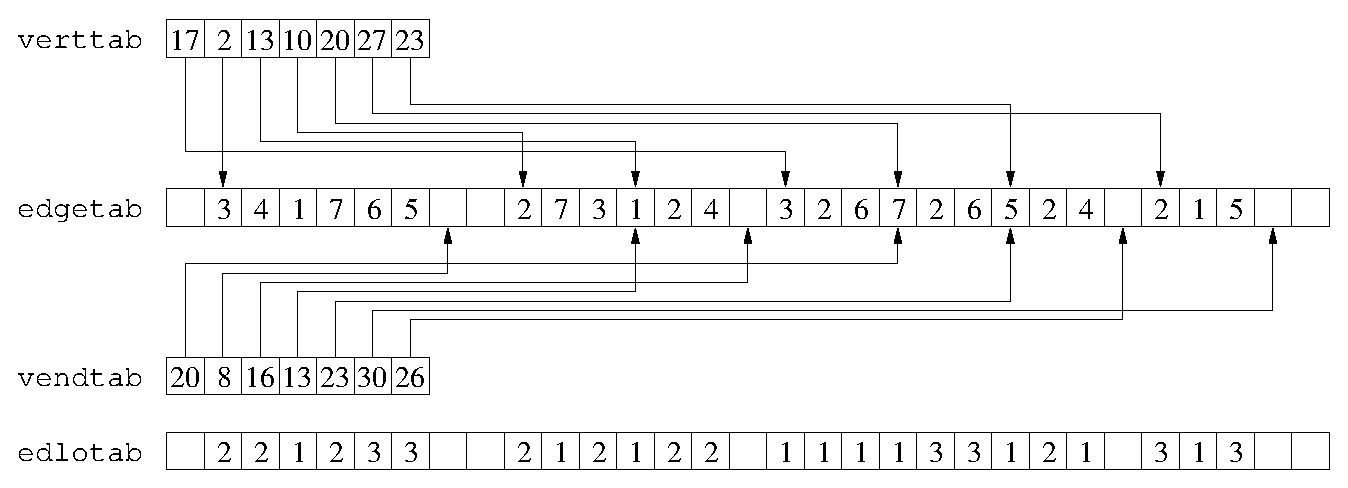
\includegraphics[scale=0.47]{s_f_gr2.eps}
\caption{Adjacency structure of the sample graph of
Figure~\protect\ref{fig-lib-graf-one} with disjoint edge and
edge load arrays. Both $\mathtt{verttax}$ and $\mathtt{vendtax}$ are
of size $\mathtt{vertnbr}$. This allows for the handling of dynamic
graphs, the structure of which can evolve with time.}
\label{fig-lib-graf-two}
\end{figure}

Dynamic graphs can be handled elegantly by using the
$\mathtt{vendtax}$ array. In order to dynamically manage graphs, one
just has to allocate $\mathtt{verttax}$, $\mathtt{vendtax}$ and
$\mathtt{edgetax}$ arrays that are large enough to contain all of the
expected new vertex and edge data. Original vertices are labeled
starting from $\mathtt{baseval}$, leaving free space at the end of the
arrays. To remove some vertex $i$, one just has to replace
$\mathtt{verttax[}i\mathtt{]}$ and
$\mathtt{vendtax[}i\mathtt{]}$ with the values of
$\mathtt{verttax[\lbt vertnbr}\lbt -1\mathtt{]}$ and
$\mathtt{vendtax[\lbt vertnbr}\lbt -1\mathtt{]}$, respectively, and
browse the adjacencies of all neighbors of former vertex
$\mathtt{vertnbr}-1$ such that all $(\mathtt{vertnbr}-1)$ indices are
turned into $i$s. Then, $\mathtt{vertnbr}$ must be decremented.

To add a new vertex, one has to fill $\mathtt{verttax[\lbt vertnbr}
-1\mathtt{]}$ and $\mathtt{vendtax[\lbt vertnbr}\lbt -1\mathtt{]}$
with the starting and end indices of the adjacency sub-array of the
new vertex. Then, the adjacencies of its neighbor vertices must also
be updated to account for it. If free space had been reserved at the
end of each of the neighbors, one just has to increment the
$\mathtt{vendtax[}i\mathtt{]}$ values of every neighbor $i$, and add
the index of the new vertex at the end of the adjacency sub-array. If
the sub-array cannot be extended, then it has to be copied elsewhere
in the edge array, and both $\mathtt{verttax[}i\mathtt{]}$ and
$\mathtt{vendtax[}i\mathtt{]}$ must be updated accordingly. With
simple housekeeping of free areas of the edge array, dynamic arrays
can be updated with as little data movement as possible.

\subsection{\texttt{Hgraph}}
\label{sec-data-hgraph}

The \texttt{Hgraph} structure holds all the information necessary to
represent and perform computations on a \textit{halo} graph. This term
refers to graphs some vertices of which are kept to preserve accurate
topological information, but are usually not subject to actual
computations. These \textit{halo vertices} are collectively referred
to as the \textit{halo} of the graph. Halo graphs are notably used in
sparse matrix reordering, where, in the process of nested dissection,
a graph is cut into three pieces: a vertex separator, and two
separated parts. Each of these parts must preserve the real degree
information attached to all their vertices, including those next to
the separator. If halo graphs were not used, the degrees of these
vertices would appear smaller than what they really are in the whole
graph. Preserving accurate degree information is essential for
algorithms such as the \textit{minimum degree} vertex ordering
method. Some vertex separation algorithms also aim at balancing halo
vertices; in this case, separators will be computed on halos, but this
information will not be preserved once a separator has been computed
on the regular vertices.

Halo graphs exhibit specific structural and topological properties,
illustrated in Figure~\ref{fig-lib-hgraf-one}. In order to distinguish
easily halo vertices from regular vertices and write efficient
algorithms, halo vertices have the highest vertex indices in the
graph. Because the degrees of halo vertices need not be preserved, no
edges connect two halo vertices; the adjacency of halo vertices is
only made of regular vertices. Also, in the adjacency arrays of
regular vertices, all non-halo vertices are placed before halo
vertices. All these properties allow one to easily induce the non-halo
graph from some halo graph, without having to create new adjacency
arrays. An additional vertex index array is present just for this
purpose.

\begin{figure}
\centering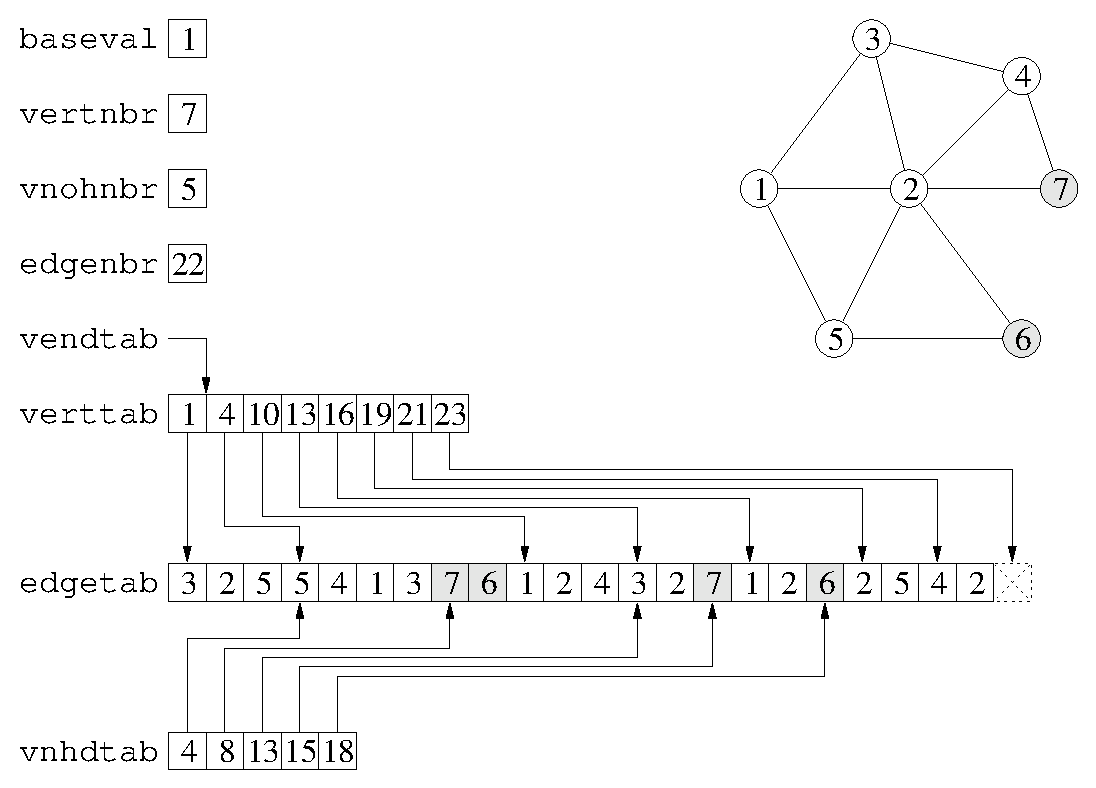
\includegraphics[scale=0.47]{m_f_gr3.eps}
\caption{Sample halo graph and its description using a compact edge
array. Numbers within vertices are vertex indices. Greyed values
are indices of halo vertices. Halo vertices have the highest indices
in the graph, and are placed last in the adjacency sub-arrays of each
non-halo vertex.}
\label{fig-lib-hgraf-one}
\end{figure}

Halo graph fields have the following meaning:
\begin{itemize}
\iteme[\texttt{s}]
Underlying source graph that contains all regular and halo
vertices. This is where to search for fields such as
$\mathtt{baseval}$, $\mathtt{vertnbr}$, $\mathtt{vertnnd}$,
$\mathtt{verttax}$, $\mathtt{vendtax}$, etc.
\iteme[\texttt{vnohnbr}]
Number of non-halo vertices in graph. Hence, $0 \leq \mathtt{vnohnbr}
\leq \mathtt{s.vertnbr}$.
\iteme[\texttt{vnhdtax}]
Array of after-last indices in $\mathtt{s.edgetax}$ of non-halo vertex
adjacency sub-arrays. Since this information only concerns non-halo
vertices, $\mathtt{vnhdtax}$ is of size $\mathtt{vnohnbr}$, not
$\mathtt{vertnbr}$.
For any non-halo vertex $i$, with $\mathtt{baseval} \leq i <
(\mathtt{vnohnbr} + \mathtt{baseval})$, the indices of the non-halo
neighbors of $i$ are stored in $\mathtt{s.edgetax}$ from $\mathtt{s.edgetax}\lbt
\mbox{\texttt{[}}\mathtt{s.verttax}\mbox{\texttt{[}}i\mbox{\texttt{]]}}$
to $\mathtt{s.edgetax}\lbt
\mbox{\texttt{[}}\mathtt{vnhdtax}\mbox{\texttt{[}}i\mbox{\texttt{]}} -
1\mbox{\texttt{]}}$, inclusive, and its halo neighbors are stored from
$\mathtt{s.edgetax}\lbt
\mbox{\texttt{[}}\mathtt{vnhdtax}\mbox{\texttt{[}}i\mbox{\texttt{]]}}$
to $\mathtt{s.edgetax}\lbt
\mbox{\texttt{[}}\mathtt{s.vendtax}\mbox{\texttt{[}}i\mbox{\texttt{]}} -
1\mbox{\texttt{]}}$, inclusive.
\iteme[\texttt{vnlosum}]
Sum of non-halo vertex loads. Hence, $0 \leq \mathtt{vnlosum}
\leq \mathtt{s.velosum}$.
\iteme[\texttt{enohnbr}]
Number of non-halo arcs in graph. Hence, $0 \leq \mathtt{enohnbr}
\leq \mathtt{s.edgenbr}$.
\end{itemize}

\subsection{\texttt{Kgraph}}
\label{sec-data-kgraph}

The \texttt{Kgraph} structure holds all the information necessary to
compute a k-way (re)mapping of some graph onto a target architecture.
Consequently, it contains a \texttt{Graph}, defined as field
\texttt{s}, and a reference to an \texttt{Arch}, through the field
\texttt{m.archptr}, as well as two \texttt{Mapping} structures: one
for the current mapping to compute, and one to store the old mapping
from which to remap. Additional information comprise data to model the
cost of remapping, and data associated with the state and cost of the
current mapping: list of frontier vertices, load of each partition
domain, plus the execution context for multi-threading execution.

The \texttt{Graph} structure is internal to the \texttt{Kgraph}
because every new \texttt{Kgraph} contains a different graph topology
(\eg, a band graph or a coarsened graph). The \texttt{Arch} is
accessed by reference because it is constant data which can be shared
by many \texttt{Kgraph}s. For the sake of consistency, the
\texttt{grafptr} fields of each mapping \texttt{m} and \texttt{r.m}
must point to \texttt{\&s}, while their two \texttt{archptr} fields
must point to the same target architecture. This redundency is the
price to pay for lighter memory management.

\subsubsection{Mappings}

The \texttt{domnorg} field, which must contain a valid domain in the
architecture \texttt{m.archptr}, is the starting point for the k-way
mapping. This domain may be smaller than the full architecture when
parallel partitioning is performed: in this case, each process may
receive a separate subgraph and sub-architecture to work on.

Each of the two mappings has its own specificities. The current
mapping, defined as field \texttt{m}, is never incomplete: all the
cells of its \texttt{m.parttax} array are non-negative values that index
a valid domain in the domain array \texttt{m.domntab}. These domains
are all subdomains of the architecture referenced through field
\texttt{m.archptr}. More restrictively, the domains attached to
non-fixed vertices must be included in \texttt{domnorg}, which may be
smaller.

The current mapping evolves with time, according to the various
algorithms that the user can activate in the strategy string. These
algorithms will create derived \texttt{Kgraph}s (\eg, band graphs or
coarsened graphs), to which mapping methods will be applied, before
the result is ported back to their parent \texttt{Kgraph}. Depending
on the kind of the derived graph, the \texttt{m.parttax} array may be
specific, but the \texttt{m.domntab} array will always be ported back
as is. Consequently, in order to save memory copying, the policy which
is implemented is that the derived \texttt{Kgraph} gets the pointer to
the \texttt{m.domntab} of its parent, while the latter is set to
\texttt{NULL}. The derived graph can therefore reallocate the array
whenever needed, without the risk of an old, invalid, pointer being
kept elsewhere. Then, when the processing of the derived
\texttt{Kgraph} ends, the most recent pointer is copied back to the
\texttt{m.domntab} field of the parent graph, and the
\texttt{m.parttax} array is updated accordingly, after which the
derived \texttt{Kgraph} can be destroyed without freeing the
pointer.

The old mapping, defined as field \texttt{r.m},
may contain incomplete mapping information: some of the cells of its
\texttt{r.m.parttax} array may be equal to \texttt{-1}, to indicate
that no prior mapping information is available (\eg, when the vertex
did not exist in the previous mapping). Since old mappings do not
change, the \texttt{r.m.domntab} field can be shared among all derived
\texttt{Kgraph}s. It is protected from double memory freeing by not
setting the \texttt{MAPPING\lbt FREE\lbt DOMN} flag in field
\texttt{r.m.flagval}.

\subsection{\texttt{Mapping}}
\label{sec-data-mapping}

The \texttt{Mapping} structure defines how individual vertices of a
\texttt{Graph} are mapped individually onto (parts of) an
\texttt{Arch}. A mapping is said \textit{complete} if all source graph
vertices are assigned to terminal target domains, \ie, individual
vertices of the target architecture, or \textit{partial} if at least
one of the source graph vertices is assigned to a target domain that
comprises more than one vertex. In the course of the graph mapping
process, the destination of source vertices are progressively refined,
from an initial target domain that usually describes the whole of the
target architecture, to terminal domains.

Since \texttt{ArchDom}, the data structure that describes target
architecture domains, is big and costly to handle (\eg, to compare if
two \texttt{ArchDom}s are identical), the handling of domains in
mapping is indirect: in the part array \texttt{parttax}, each vertex
is assigned an integer domain index that refers to a domain located in
the domain array \texttt{domntab}. Hence, when two graph vertices have
the same index in \texttt{parttax}, they belong to the same domain and
induce no communication cost. However, the opposite is false: two
vertices may have a different index in \texttt{parttax} and yet belong
to the same target domain. This is for instance the case when one of
the vertices is a fixed vertex that has been set to a specific
terminal domain at initialization time, and one of its neighbors is
successively mapped to smaller and smaller subdomains that eventually
amount to the same terminal domain.

In the case of a remapping, the mapping information regarding the
former placement of the vertices may be incomplete, \eg, because the
vertex did not exist before. Such a mapping is said to be
\textit{incomplete}. It is characterized by the fact that some cells
of the \texttt{parttax} array are equal to \texttt{-1}, to indicate an
unknown terminal domain number. To allow for this, the mapping must
have the \texttt{MAPPING\lbt INCOMPLETE} flag set. Incomplete mappings
are only valid when holding remapping information; new mappings being
computed must have all their \texttt{parttax} cells set with
non-negative values that point to valid domains in the
\texttt{domntab} array. New mappings can therefore only be partial or
complete.

When a mapping is initialized, all \texttt{parttax} values for
non-fixed vertices are set to index~$0$, and \texttt{domntab[0]} is
set to the root domain for the mapping. In the general case for
centralized mapping, the initial domain is equal to
\texttt{archDomFrst(archptr)}. However, when a centralized mapping
process is launched as a part of a distributed mapping process, the
initial domain may be a subset of the whole target architecture.

There is no obligation for the \texttt{domntab} array to contain only
one instance of some target domain. On the contrary, as described
above, the same domain may appear at least twice: once for fixed
vertices, and once for non-fixed vertices on which mapping algorithms
are applied. However, for efficiency reasons (\eg, avoiding to compute
vertex distances that are equal to zero), it is preferable that
duplicate domains are avoided in the \texttt{domntab} array. This is
the case by nature with recursive bipartitioning, as the domains
associated with branches of the biparitioning tree are all distinct.

Making the distinction between fixed and non-fixed vertices, which is
relevant to mapping algorithms, is not in the scope of the
\texttt{Mapping} data structure, which only represents a global
state. This is why no data related to fixed vertices is explicitly
present in the mapping itself (it may be found, \eg, in the
\texttt{Kgraph} data structure).
However, for handling fixed vertices in an efficient way, the
semantics of the \texttt{Mapping} data structure is that all domains
that are associated with fixed vertices must be placed first in the
\texttt{domntab} array. The purpose of this separation is because,
when the imbalance of a mapping is computed, the loads of non-fixed
vertices that belong to some (partial) domain and of fixed vertices
that belong to domains that are subdomains of this domain have to be
aggregated. This aggregation procedure is made easier if both types of
domains are kept separate. For efficiency reasons, fixed domains
should appear only once in the fixed part of \texttt{domntab}.
\\

The \texttt{Mapping} structure is mainly used within the
\texttt{Kgraph} structure, which contains two instances of it: one for
the current mapping to be computed, and one for the old mapping, in
the case of remapping. The building of a \texttt{Kgraph} from another
one (\eg, when creating a band graph or a coarsened graph) may lead to
situations in which some \texttt{Mapping} arrays may be re-used, and
thus should not be freed when the derived \texttt{Mapping} is
freed. This is why the \texttt{Mapping} structure contains flags to
record whether its arrays should be freed or not. These flags are the
following:
\begin{itemize}
\iteme[\texttt{MAPPINGFREEDOMN}]
  Set if the domain array has to be freed when the mapping is freed. A
  common case for sharing the domain array is when a coarser
  \texttt{Kgraph} is computed: the domain array of the coarse old
  mapping can re-use that of the fine old mapping.
\iteme[\texttt{MAPPINGFREEPART}]
  Set if the part array has to be freed when the mapping is freed. A
  common case for sharing the part array is when the user part array
  is kept as the part array for the initial \texttt{Kgraph} current
  mapping structure.
\end{itemize}

The main fields of the \texttt{Mapping} data structure are the following:
\begin{itemize}
\iteme[\texttt{flagval}]
  Set of flags indicating whether the \texttt{parttax} and
  \texttt{domntab} have to be freed on exit.
\iteme[\texttt{grafptr}]
  Pointer to the \texttt{Graph} associated with the mapping, that
  gives access to the base value \texttt{grafptr->\lbt baseval} and
  the number of source vertices \texttt{grafptr->\lbt vertnbr}.
\iteme[\texttt{archptr}]
  Pointer to the \texttt{Arch} associated with the mapping, that is
  necessary to perform all distance computations on the mapping.
\iteme[\texttt{parttax}]
  Based array of \texttt{Anum}s, of size \texttt{grafptr->\lbt
  vertnbr}, that provides the index of the target domains onto which
  all graph vertices are currently mapped. Indices are un-based.
\iteme[\texttt{domntab}]
  Un-based array of \texttt{ArchDom}s, of size \texttt{domnmax}, that
  stores the target domains to which source graph vertices are
  indirectly associated through the \texttt{parttax} array.
\iteme[\texttt{domnnbr}]
  Number of target domain slots currently used in
  \texttt{domntab}. After a mapping is initialized, $1 \leq
  \mbox{\texttt{domnnbr}} < \mbox{\texttt{domnmax}}$, because source
  graph vertices must be associated to some domain, hence
  \texttt{domntab} should at least contain one domain.
\iteme[\texttt{domnnbr}]
  Number of target domain slots currently used in
  \texttt{domntab}.
\iteme[\texttt{domnmax}]
  Size of the \texttt{domntab} array.
\iteme[\texttt{mutedat}]
  When multi-threading is activated, allows to create critical
  sections to update the mapping data in a thread-safe manner.
\end{itemize}

\subsection{\texttt{Order}}
\label{sec-data-order}

Orderings are data structures used in \scotch\ to represent
fill-minimizing block orderings of adjacency matrices represented as
graphs. A block ordering, contained in the \texttt{Order} data
structure, is defined by an inverse permutation, which provides the
old indices of the reordered vertices, and a column block
decomposition of the reordered matrix, to help performing more
efficient block computations at the solving stage.

Inverse permutations are used, instead of direct permutations, because
their processing is more local: when ordering some subgraph, the only
ordering information to provide is the un-based start index, usually
called \texttt{ordenum}, in the inverse permutation vector, usually
called \texttt{peritab}, while the \texttt{vnumtax} array of the
\texttt{Graph} structure holds the values of the vertex indices to
write in the sub-array of \texttt{peritab} starting at index
\texttt{ordenum}, of a size equal to the number of concerned vertices
in the \texttt{Graph}. Once an ordering is computed, it is
straightforward to compute the direct permutation \texttt{permtab}
from the inverse permutation \texttt{peritab}, in case it is needed.

The column block decomposition is defined as a tree structure, whose
nodes, of type \texttt{Order\lbt Cblk}, represent column blocks
containing consecutive, reordered vertices. A tree node may have
ordered children nodes, which represent the decomposition of a column
block into sub-column blocks, \eg, when a subdomain is decomposed into
two separated subdomains and a separator.

The main fields of the \texttt{Order} data structure are the
following:
\begin{itemize}
\iteme[\texttt{flagval}]
Flag that indicates whether the \texttt{peritab} inverse permutation
array has to be freed on exit.
\iteme[\texttt{baseval}]
Base value for inverse permutation values.
\iteme[\texttt{vnodnbr}]
Number of vertex nodes in the ordering. When the associated graph
structure is a \texttt{Graph}, this number is equal to its
\texttt{vertnbr} field; when it is a \texttt{Mesh}, it is equal to
its \texttt{vnodnbr} field.
\iteme[\texttt{treenbr}]
Number of tree nodes in the ordering. This number is equal to $1$ when
only the root tree node is present, and is incremented each time a new
tree node is added to the tree structure.
\iteme[\texttt{cblknbr}]
Number of column blocks in the ordering. This number is equal to $1$
when only the root tree node is present. When some column block
is decomposed into $c$ sub-column blocks, it is increased by $(c-1)$,
since this represents the number of additional column blocks in the
structure.
\iteme[\texttt{rootdat}]
Root column block of the ordering. This structure, of type
\texttt{Order\lbt Cblk}, is initialized to contain all \texttt{Graph}
vertices, or \texttt{Mesh} vertex nodes, in a single column block,
after which reordering algorithms are applied and lead to the creation
of sub-column blocks, \eg, in the case of nested dissection.
\iteme[\texttt{peritab}]
Pointer to the inverse permutation array.
\iteme[\texttt{mutedat}]
Mutual exclusion lock. When multi-threading is activated, it allows to
create critical sections to update the ordering data in a thread-safe
manner.
\end{itemize}

\subsubsection{\texttt{OrderCblk}}
\label{sec-data-order-cblk}

Column blocks are sets of reordered unknowns which are likely to be
processed efficiently together when solving the linear system, \eg,
using BLAS block computation routines. The column block decomposition
of the reordered matrix is represented as a tree whose nodes are
instances of the \texttt{OrderCblk} data structure. The column block
decomposition tree will be used to create the block elimination tree
of the unknowns of the linear system, which amounts to linking each
column block to a father block. This building is performed by the
\texttt{order\lbt Tree()} routine.

A column block tree node \texttt{OrderCblk} is defined by its type
(\ie, whether it is a leaf, a nested dissection node, etc.), its width
(\ie, the number of node vertices it contains), and, if it is not a
leaf, the description of the sub-column blocks it contains.
The main fields of the \texttt{OrderCblk} data structure are the
following:
\begin{itemize}
\iteme[\texttt{typeval}]
  Set of flags that define the nature of the column block tree
  node. They must be the same as the distributed column block tree
  node flags of the \texttt{Dorder\lbt Cblk} distributed column block
  data structure. Consequently, these flags must be separate bits, so
  that values can be or-ed (especially, concerning \texttt{ORDER\lbt
  CBLK\lbt LEAF} in \texttt{hdgraph\lbt Order\lbt Nd()}).
  These flags are the following:
  \begin{itemize}
  \iteme[\texttt{ORDERCBLKLEAF}]
    Leaf column block (before it is subdivided into sub-column blocks,
    or definitely). In this case, the other fields of the column block
    tree node are such that $\texttt{cblknbr} = 0$ and
    $\texttt{cblktab} = \texttt{NULL}$.
  \iteme[\texttt{ORDERCBLKNEDI}]
    Nested-dissection separator tree node. The separator is always
    the last sub-column block. Hence, if the separator is not empty,
    the node has three sub-column blocks (hence $\texttt{cblknbr} =
    3$), while, if the separator is empty, the column block tree node
    has only two sub-column blocks (hence $\texttt{cblknbr} = 2$).
    None of the separated parts can be empty (else, the tree node
    would be of type \texttt{ORDER\lbt CBLK\lbt SEQU}).
  \iteme[\texttt{ORDERCBLKDICO}]
    Disconnected components tree node. It contains an arbitrary number
    (always strictly greater than~$1$) of sub-column blocks, which
    represent disconnected components to be ordered
    independently. Since the sub-column blocks are not connected,
    their father in the elimination tree will not be the column block
    tree node itself, but its father (or none if the column block is
    the root column block, \ie, the \texttt{rootdat} field of the
    \texttt{Order} data structure).
  \iteme[\texttt{ORDERCBLKSEQU}]
    Sequential tree node. It contains an arbitrary number
    (always strictly greater than~$1$) of sub-column blocks, which
    represent mutually dependent blocks. Consequently, the father of
    each sub-column block in the elimination tree will be the next
    sub-column block, except for the last sub-column block, whose
    father will be the column block itself.
  \end{itemize}
\iteme[\texttt{vnodnbr}]
  Number of nodes (\ie, vertices) contained in the column block. If
  the column block has sub-column blocks, the sum of all the
  \texttt{vnodnbr} values of the sub-column blocks must be equal to
  the \texttt{vnodnbr} of the column block.
\iteme[\texttt{cblknbr}]
  Number of sub-column blocks. If the column block is a leaf,
  $\texttt{cblknbr} = 0$ and $\texttt{cblktab} = \texttt{NULL}$.
\iteme[\texttt{cblktab}]
  Array of \texttt{cblknbr} structures of type \texttt{DorderCblk},
  which hold the data about the sub-column blocks if the column block
  is not a leaf. \texttt{cblktab} has to be freed on exit.
\end{itemize}
                                  % Data stuctures explanation
%%%%%%%%%%%%%%%%%%%%%%%%%%%%%%%%%%%%
%                                  %
% Title   : m_c.tex                %
% Subject : Maintenance manual of  %
%           Scotch                 %
%           Code explanations      %
% Author  : Francois Pellegrini    %
%                                  %
%%%%%%%%%%%%%%%%%%%%%%%%%%%%%%%%%%%%

\section{Code explanations}
\label{sec-code}

This section explains some of the most complex algorithms implemented
in \scotch\ and \ptscotch.

\subsection{\texttt{dgraphCoarsenBuild()}}

The \texttt{dgraphCoarsenBuild()} routine creates a coarse distributed
graph from a fine distributed graph, using the result of a distributed
matching. The result of the matching is available on all MPI processes
as follows:
\begin{itemize}
\iteme[\texttt{coardat.\lbt multlocnbr}]
  The number of local coarse vertices to be created.
\iteme[\texttt{coardat.\lbt multloctab}]
  The local multinode array. For each local coarse vertex to be
  created, it contains two values. The first one is always positive,
  and represents the global number of the first local fine vertex to
  be mated. The second number can be either positive or negative. If
  it is positive, it represents the global number of the second local
  fine vertex to be mated. If it is negative, its opposite, minus two,
  represents the local edge number pointing to the remote vertex to be
  mated.
\iteme[\texttt{coardat.\lbt procgsttax}]
  Array (restricted to ghost vertices only) that records on which
  process is located each ghost fine vertex.
\end{itemize}

\subsubsection{Creating the fine-to-coarse vertex array}

In order to build the coarse graph, one should create the array that
provides the coarse global vertex number for all fine vertex ends
(local and ghost). This information will be stored in the
\texttt{coardat.\lbt coargsttax} array.

Hence, a loop on local multinode data fills
\texttt{coardat.\lbt coargsttax}. The first local multinode vertex
index is always local, by nature of the matching algorithm.
If the second vertex is local too, \texttt{coardat.\lbt coargsttax} is
filled instantly. Else, a request for the global coarse vertex number
of the remote vertex is forged, in the \texttt{vsnddattab} array,
indexed by the current index \texttt{coarsndidx} extracted from the
neighbor process send index table \texttt{nsndidxtab}. Each request
comprises two numbers: the global fine number of the remote vertex for
which the coarse number is seeked, and the global number of the
coarse multinode vertex into which it will be merged.

Then, an all-to-all-v data exchange by communication takes place,
using either the \texttt{dgraph\lbt Coarsen\lbt Build\lbt Ptop()} or
\texttt{dgraph\texttt Coarsen\lbt Build\lbt Coll()} routines.  Apart
from the type of communication they implement (either point-to-point
or collective), these routines do the same task: they process the
pairs of values sent from the \texttt{vsnddattab} array. For each pair
(the order of processing is irrelevant), the \texttt{coargsttax} array
of the receiving process is filled-in with the global multinode value
of the remotely mated vertex. Hence, at the end of this phase, all
processes have a fully valid local part of the \texttt{coargsttax}
array; no value should remain negative (as set by default). Also, the
\texttt{nrcvidxtab} array is filled, for each neighbor process, of the
number of data it has sent. This number is preserved, as it will serve
to determine the number of adjacency data to be sent back to each
neighbor process.

Then, data arrays for sending edge adjacency are filled-in. The
\texttt{ercvdsptab} and \texttt{ercvcnttab} arrays, of size
\texttt{procglbnbr}, are computed according to the data stored in
\texttt{coardat.\lbt dcntglbtab}, regarding the number of vertex- and
edge-related data to exchange.

By way of a call to \texttt{dgraphHaloSync()}, the ghost data of the
\texttt{coargsttax} array are exchanged.

Then, \texttt{edgelocnbr}, an upper bound on the number of local
edges, as well as \texttt{ercvdatsiz} and \texttt{esnddatsiz}, the
edge receive and send array sizes, respectively.

Then, all data arrays for the coarse graph are allocated, plus the
main adjacency send array \texttt{esnddsptab}, its receive counterpart
\texttt{ercvdattab}, and the index send arrays \texttt{esnddsptab} and
\texttt{esndcnttab}, among others.

Then, adjacency send arrays are filled-in. This is done by performing
a loop on all processes, within which only neighbor processes are
actually considered, while index data in \texttt{esnddsptab} and
\texttt{esndcnttab} is set to $0$ for non-neighbor processes. For each
neighbor process, and for each vertex local which was remotely mated
by this neighbor process, the vertex degree is written in the
\texttt{esnddsptab} array, plus optionally its load, plus the edge
data for each of its neighbor vertices: the coarse number of its end,
obtained through the \texttt{coargsttax} array, plus optionally the
edge load. At this stage, two edges linking to the same coarse
multinode will not be merged together, because this would have
required a hash table on the send side. The actual merging will be
performed once, on the receive side, in the next stage of the
algorithm.

\subsection{\texttt{dgraphFold()} and \texttt{dgraphFoldDup()}}

The \texttt{dgraph\lbt Fold()} routine creates a ``folded''
distributed graph from the input distributed graph. The folded graph
is such that it spans across only one half of the processing elements
of the initial graph (either the first half, or the second half). The
purpose of this folding operation is to preserve a minimum average
number of vertices per processing element, so that communication cost
is not dominated by message start-up time. In case of an odd number
of input processing elements, the first half of them is always bigger
that the second.

The \texttt{dgraph\lbt Fold\lbt Dup()} routine creates two folded
graphs: one for each half. Hence, each processing element hosting the
initial graph will always participate in hosting a new graph, which
will depend on the rank of the processing element. When the MPI
implementation supports multi-threading, and multi-threading is
activated in \scotch, both folded graphs are created concurrently.

The folding routines are based on the computation of a set of
(supposedly efficient) point-to-point communications between the
\textit{sender processes}, which will not retain any graph data, and
the \textit{receiver processes}, which will host the folded
graph. However, in case of unbalanced vertex distributions, overloaded
receiver processes (called \textit{sender receiver processes}) may
also have to send their extra vertices to underloaded receiver
processes. A receiver process may receive several chunks of vertex
data (including their adjacency) from several sender processes. Hence,
folding amounts to a redistribution of vertex indices across all
receiver processes. In particular, end vertex indices have to be
renumbered according to the global order in which the chunks of data
are exchanged. This is why the computation of these exchanges, by way
of the \texttt{dgraph\lbt Fold\lbt Comm()} routine, has to be fully
deterministic and reproducible across all processing elements, to
yield consistent communication data. The result of this computation
is a list of point-to-point communications (either all sends or
receives) to be performed by the calling process, and an array of
sorted global vertex indices, associated with vertex index adjustment
values, to convert global vertex indices in the adjacency of the
initial graph into global vertex indices in the adjacency of the
folded graph. This array can be used, by way of dichotomy search, to
find the proper adjustment value for any end vertex number.

To date, the \texttt{dgraph\lbt Redist()} routine is not based on a
set of point-to-point communications, but collectives. It could well
be redesigned to re-use the mechanisms implemented here, with relevant
code factorization.

\subsubsection{\texttt{dgraphFoldComm()}}

The \texttt{dgraphFoldComm()} routine is at the heart of the folding
operation. It computes the sets of point-to-point communications
required to move vertices from the sending half of processing elements
to the receiving half, trying to balance the folded graph as much as
possible in terms of number of vertices. For receiver processes, it
also computes the data needed for the renumbering of the adjacency
arrays of the graph chunks received from sender (or sender receiver)
processes.

It is to be noted that the end user and the \scotch\ algorithms may
have divergent objectives regarding balancing: in the case of a
weighted graph representing a computation, where some vertices bear a
higher load than others, the user may want to balance the load of its
computations, even if it results in some processing elements having
less vertices than others, provided the sums of the loads of these
vertices are balanced across processing elements. On the opposite, the
algorithms implemented in \scotch\ operate on the vertices themselves,
irrespective of the load values that is attached to them (save for
taking them into account for computing balanced partitions). Hence,
what matters to \scotch\ is that the number of vertices is balanced
across processing elements. Whenever \scotch\ is provided with an
unbalanced graph, it will try to rebalance it in subsequent
computations (\eg, folding). However, the bulk of the work, on the
initial graph, will be unbalanced according to the user's
distribution.

During a folding onto one half of the processing elements, the
processing elements of the other half will be pure
senders, that need to dispose of all of their vertices and
adjacency. Processing elements of the first half will likely be
receivers, that will take care of the vertices sent to them by
processing elements of the other half. However, when a processing
element in the first half is overloaded, it may behave as a
sender rather than a receiver, to dispose of its extra vertices and
send it to an underloaded peer.

The essential data that is produced by the \texttt{dgraph\lbt Fold\lbt
Comm()} routine for the calling processing element is the following:
\begin{itemize}
\iteme[\texttt{commmax}]
  The maximum number of point-to-point communications that can be
  performed by any processing element. The higher this value, the
  higher the probability to spread the load of a highly overloaded
  processing element to (underloaded) receivers. In the extreme case
  where all the vertices are located on a single processing element,
  $(\mbox{\texttt{procglbnbr}} - 1)$ communications would be
  necessary. To prevent such a situation, the number of communications
  is bounded by a small number, and receiver processing elements can
  be overloaded by an incoming communication. The algorithm strives to
  provide a \textit{feasible} communication scheme, where the current
  maximum number of communications per processing element suffices to
  send the load of all sender processing elements. When the number of
  receivers is smaller than the number of senders (in practice, only
  by one, in case of folding from an odd number of processing
  elements), at least two communications have to take place on some
  receiver, to absorb the vertices sent. The initial maximum number of
  communications is defined by \texttt{DGRAPH\lbt FOLD\lbt COMM\lbt
  NBR};
\iteme[\texttt{commtypval}]
  The type of communication and processing that the processing element
  will have to perform: either as a sender, a receiver, or a sender
  receiver. Sender receivers will keep some of their vertex data, but
  have to send the rest to other receivers. Sender receivers do send
  operations only, and never receive data from a sender;
\iteme[\texttt{commdattab}]
  A set of slots, of type \texttt{Dgraph\lbt Fold\lbt Comm\lbt Data},
  that describe the point-to-point communications that the processing
  element will initiate on its side. Each slot contains the number of
  vertices to send or receive, and the target or source process index,
  respectively;
\iteme[\texttt{commvrttab}]
  A set of values associated to each slot in \texttt{comm\lbt dat\lbt
  tab}, each of which contains the global index number of the first
  vertex of the graph chunk that will be transmitted;
\iteme[\texttt{proccnttab}]
  For receiver processes only, the count array of same name of the
  folded distributed graph structure;
\iteme[\texttt{vertadjnbr}]
  For receiver processes only, the number of elements in the dichotomy
  array \texttt{vert\lbt adj\lbt tab};
\iteme[\texttt{vertadjtab}]
  A sorted array of global vertex indices. Each value represent the
  global start index of a graph chunk that will been exchanged (or
  which will remain in place on a receiver processing element);
\iteme[\texttt{vertdlttab}]
  The value which has to be added to the indices of the vertices in
  the corresponding chunk represented in \texttt{vert\lbt adj\lbt
  tab}. This array and the latter serve to find, by dichotomy, to
  which chunk an end vertex belongs, and modify its global vertex
  index in the edge array in the receiver processing element. Although
  \texttt{vert\lbt adj\lbt tab} and \texttt{vert\lbt dlt\lbt tab}
  contain strongly related information, they are separate arrays, for
  the sake of memory locality. Indeed, \texttt{vert\lbt adj\lbt tab}
  will be subject to a dichotomy search, involving many memory reads,
  before the proper index is found and a single value is retrieved
  from the \texttt{vert\lbt dlt\lbt tab} array.
\end{itemize}

The first stage of the algorithm consists in sorting a global process
load array in ascending order, in two parts: the sending half, and the
receiving half. These two sorted arrays will contain the source
information which the redistribution algorithm will use. Because the
receiver part of the sort array can be modified by the algorithm, it
is recomputed whenever \texttt{commmax} is incremented. It is the same
for \texttt{sort\lbt snd\lbt bas}, the index of the first non-empty
sender in the sort array.
\\

In a second stage, the algorithm will try to compute a valid
communication scheme for vertex redistribution, using as many as
\texttt{commmax} communications (either sends or receives) per
processing element. During this outermost loop, if a valid
communication scheme cannot be created, then \texttt{commmax} is
incremented and the communication scheme creation algorithm is
restarted. The initial value for \texttt{commmax} is
\texttt{DGRAPH\lbt FOLD\lbt COMM\lbt NBR}.

The construction of a valid communication scheme is performed within
an intermediate loop. At each step, a candidate sender process is
searched for: either a sender process which has to dispose of all of
its vertices, or an overloaded receiver process, depending on which
has the biggest number of vertices to send. If candidate senders can
no longer be found, the stage has succeeded with the current value of
\texttt{commmax}; if a candidate sender has been found but a candidate
receiver has not, the outermost loop is restarted with an incremented
\texttt{commmax} value, so as to balance loads better.

Every time a sender has been found and one or more candidate receivers
exist, an inner loop creates as many point-to-point communications as
to spread the vertices in chunks, across one or more available
receivers, depending on their capacity (\ie, the number of vertices
they can accept). If the selected sender is a sender receiver, the
inner loop will try to interleave small communications from pure
senders with communications of vertex chunks from the selected
sender receiver. The purpose of this interleaving is to reduce the
number of messages per process: a big message from a sender receiver
is likely to span across several receivers, which will then perform
only a single receive communication. By interleaving a small
communication on each of the receivers involved, the latter will only
have to perform one more communication (\ie, two communications only),
and the interleaved small senders will be removed off the list,
reducing the probability that afterwards many small messages will sent
to the same (possibly eventually underloaded) receiver.
\\

In a third stage, all the data related to chunk exchange, which was
recorded in a temporary form in the \texttt{vertadjtab},
\texttt{vertdlttab} and \texttt{slotsndtab} arrays, is compacted to
remove empty slots and to form the final \texttt{vertadjtab} and
\texttt{vertdlttab} arrays to be used for dichotomy search.
\\

The data structures that are used during the computation of
vertex global index update arrays are the following:
\begin{itemize}
\iteme[\texttt{vertadjtab} and \texttt{vertdlttab}]
  These two arrays have been presented above. They are created only
  for receiver processes, and will be filled concurrently. They are of
  size $((\mbox{\texttt{commmax}} + 1) * \mbox{\texttt{orgprocnbr}})$,
  because in case a process is a sender receiver, it has to use a
  first slot to record the vertices it will keep locally, plus
  \texttt{commmax} for outbound communications.  During the second
  stage of the algorithm, for some slot \texttt{i},
  \texttt{vertadjtab[i]} holds the start global index of the chunk of
  vertices that will be kept, sent or received, and
  \texttt{vertdlttab[i]} holds the number of vertices that will be
  sent or received.  During the third stage of the algorithm, all this
  data will be compacted, to remove empty slots. After this,
  \texttt{vertadjtab} will be an array of global indices used for
  dichotomy search in \texttt{dgraph\lbt Fold()}, and
  \texttt{vertdlttab[i]} will hold the adjustment value to apply to
  vertices whose global indices are comprised between
  \texttt{vertadjtab[i]} and \texttt{vertadjtab[i+1]}.
\iteme[\texttt{slotsndtab}]
  This array only has cells for receiver-slide slots, hence a size of
  $((\mbox{\texttt{commmax}} + 1) * \mbox{\texttt{procfldnbr}})$
  items. During the second stage of the algorithm, it is filled so
  that, for any non-empty communication slot \texttt{i} in
  \texttt{vertadjtab} and \texttt{vertdlttab}, representing a receive
  operation, \texttt{slotsndtab[i]} is the slot index of the
  corresponding send operation. During the third stage of the
  algorithm, it is used to compute the accumulated vertex indices
  across processes.
\end{itemize}

Here are some examples of redistributions that are computed by the
\texttt{dgraph\lbt Fold\lbt Comm()} routine.

\begin{lstlisting}
orgvertcnttab = { 20, 20, 20, 20, 20, 20, 20, 1908 }
partval = 1
vertglbmax = 1908
Proc [0] (SND) 20 -> 0 : { [4] <- 20 }
Proc [1] (SND) 20 -> 0 : { [5] <- 20 }
Proc [2] (SND) 20 -> 0 : { [6] <- 20 }
Proc [3] (SND) 20 -> 0 : { [6] <- 20 }
Proc [4] (RCV) 20 -> 512 : { [0] -> 20 }, { [7] -> 472 }
Proc [5] (RCV) 20 -> 512 : { [1] -> 20 }, { [7] -> 472 }
Proc [6] (RCV) 20 -> 512 : { [2] -> 20 }, { [7] -> 452 }, { [3] -> 20 }
Proc [7] (RSD) 1908 -> 512 : { [4] <- 472 }, { [5] <- 472 }, { [6] <- 452 }
commmax = 4
commsum = 14
\end{lstlisting}
We can see in the listing above that some interleaving took place
on the first receiver (proc.~4) before the sender receiver (proc.~7)
did its first communication towards it.

\begin{lstlisting}
orgvertcnttab = { 0, 0, 0, 20, 40, 40, 40, 100 }
partval = 1
vertglbmax = 100
Proc [0] (SND) 0 -> 0 : 
Proc [1] (SND) 0 -> 0 : 
Proc [2] (SND) 0 -> 0 : 
Proc [3] (SND) 20 -> 0 : { [4] <- 20 }
Proc [4] (RCV) 40 -> 60 : { [3] -> 20 }
Proc [5] (RCV) 40 -> 60 : { [7] -> 20 }
Proc [6] (RCV) 40 -> 60 : { [7] -> 20 }
Proc [7] (RSD) 100 -> 60 : { [5] <- 20 }, { [6] <- 20 }
commmax = 4
commsum = 6
\end{lstlisting}
In the latter case, one can see that the pure sender that has been
interleaved (proc.~3) sufficed to fill-in the first receiver
(proc.~4), so the first communication of the sender receiver (proc.~7)
was towards the next receiver (proc.~5).
                                  % Code explanation
%%%%%%%%%%%%%%%%%%%%%%%%%%%%%%%%%%%%
%                                  %
% Title   : m_m.tex                %
% Subject : Maintenance manual of  %
%           Scotch                 %
%           Procedures             %
% Author  : Francois Pellegrini    %
%                                  %
%%%%%%%%%%%%%%%%%%%%%%%%%%%%%%%%%%%%

\section{Procedures for new developments and release}

\subsection{Adding methods to the \libscotch\ library}
\label{sec-method}

The \libscotch\ has been carefully designed to allow external
contributors to add their new partitioning or ordering methods, and
to use \scotch\ as a testbed for them.

\subsubsection{What to add}

There are currently seven types of methods which can be added:
\begin{itemize}
\item
k-way graph mapping methods, in module \texttt{kgraph};
\item
graph bipartitioning methods by means of edge separators, in module
\texttt{bgraph}, used by the mapping method by dual recursive
bipartitioning, implemented in \texttt{kgraph\_\lbt map\_\lbt rb.[ch]};
\item
graph ordering methods, in module \texttt{hgraph};
\item
graph separation methods by means of vertex separators, in module
\texttt{vgraph}, used by the nested dissection ordering method
implemented in \texttt{hgraph\_\lbt order\_\lbt nd.[ch]};
\item
mesh ordering methods, in module \texttt{hmesh};
\item
mesh separation methods with vertex separators, in module
\texttt{vmesh}, used by the nested dissection ordering method
implemented in \texttt{hmesh\_\lbt order\_\lbt nd.[ch]};
\item
graph partitioning methods with separator overlap, in module
\texttt{wgraph}.
\end{itemize}
Every method of these seven types operates on instances of augmented
graph structures that contain, in addition to the graph topology,
data related to the current state of the partition or of the
ordering. For instance, all of the graph bipartitioning methods
operate on an instance of a \texttt{Bgraph}, defined in \texttt{bgraph.h},
and which contains fields such as \texttt{compload0}, the current load
sum of the vertices assigned to the first part, \texttt{commload}, the
load sum of the cut edges, etc.

In order to understand better the meaning of each of the fields
used by some augmented graph or mesh structure, contributors can read
the code of the consistency checking routines, located in files ending
in \texttt{\_check.c}\enspace, such as \texttt{bgraph\_check.c} for a
\texttt{Bgraph} structure. These routines are regularly called during the
execution of the debug version of \scotch\ to ease bug tracking. They
are time-consuming but proved very helpful in the development and
testing of new methods.

\subsubsection{Where to add}

Let us assume that you want to code a new graph separation
routine. Your routine will operate on a \texttt{Vgraph} structure, and
thus will be stored in files called \texttt{vgraph\_\lbt separate\_
xy\lbt .[ch]}, where \texttt{xy} is a two-letter reminder of the name
of your algorithm. Look into the \libscotch\ source directory for
already used codenames, and pick a free one.
In case you have more that one single source file, use extended names,
such as \texttt{vgraph\_\lbt separate\_\lbt xy\_\lbt subname\lbt
.[ch]}\enspace .

In order to ease your coding, copy the files of a simple and already
existing method and use them as a pattern for the interface of your
new method. Some methods have an optional parameter data structure,
others do not. Browse through all existing methods to find the one
that looks closest to what you want.

Some methods can be passed parameters at run time from the strategy
string parser. These parameters can be of fixed types only. These
types are:
\begin{itemize}
\item
an integer (\texttt{int}) type,
\item
a floating-point (\texttt{double}) type,
\item
an enumerated (\texttt{char}) type: this type is used to make a
choice among a list of single character values, such as
``\texttt{yn}''. It is more readable than giving integer numerical
values to method option flags,
\item
a strategy (\scotch\ \texttt{Strat} type): a method can be passed a
sub-strategy of a given type, which can be run on an augmented graph
of the proper type. For instance, the nested dissection method in
\texttt{hgraph\_\lbt order\_\lbt nd\lbt .c} uses a graph separation
strategy to compute its vertex separators.
\end{itemize}

\subsubsection{Declaring the new method to the parser}

Once the new method has been coded, its interface must be known to the
parser, so that it can be used in strategy strings. All of this is
done in the module strategy method files, the name of which always end
in \texttt{\_st.[ch]}, that is, \texttt{vgraph\_\lbt separate\_\lbt st.[ch]}
for the \texttt{vgraph} module. Both files are to be updated.

In the header file {*\_st.h}, a new identifier must be created for the
new method in the \texttt{St\lbt Method\lbt Type} enumeration type,
preferrably placed in alphabetical order.

In file {*\_st.c}, there are several places to update.
First, in the beginning of the module file, the header file of the new
method, \texttt{vgraph\_\lbt separate\_\lbt xy.h} in this example,
must be added in alphabetical order to the list of included method
header files.

Then, if the new method has parameters, an instance of the method
parameter structure must be created, which will hold the default
values for the method. This is in fact a \texttt{union} structure,
of the following form:
{\tt\begin{verbatim}
static union {
  VgraphSeparateXyParam     param;
  StratNodeMethodData       padding;
} vgraphseparatedefaultxy = { { ... } };
\end{verbatim}}
where the dots should be replaced by the list of default values of the
fields of the \texttt{Vgraph\lbt Separate\lbt Xy\lbt Param} structure.
Note that the size of the \texttt{Strat\lbt Node\lbt Method\lbt Data}
structure, which is used as a generic padding structure, must always
be greater than or equal to the size of each of the parameter
structures. If your new parameter structure is larger, you will have
to update the size of the \texttt{Strat\lbt Node\lbt Method\lbt Data}
type in file \texttt{parser.h}\enspace. The size of the \texttt{Strat\lbt
Node\lbt Method\lbt Data} type does not depend directly on the size of
the parameter structures (as could have been done by making it an union
of all of them) so as to to reduce the dependencies between the files
of the library. In most cases, the default size is sufficient, and a
test is added in the beginning of all method routines to ensure it is
the case in practice.

Finally, the first two method tables must be filled accordingly. In the
first one, of type \texttt{Strat\lbt Method\lbt Tab}, one must add a new
line linking the method identifier to the character code used to name
the method in strategy strings (which must be chosen among all of
the yet unused letters), the pointer to the routine, and the pointer
to the above default parameter structure if it exists (else, a
\texttt{NULL} pointer must be provided).
In the second one, of type \texttt{Strat\lbt Param\lbt Tab}, one must add
one line per method parameter, giving the identifier of the method,
the type of the parameter, the name of the parameter in the strategy
string, the base address of the default parameter structure, the
actual address of the field in the parameter structure (both fields
are required because the relative offset of the field with respect to
the starting address of the structure cannot be computed at
compile-time), and an optional pointer that references either the
strategy table to be used to parse the strategy parameter (for
strategy parameters) or a string holding all of the values of the
character flags (for an enumerated type), this pointer being set to
\texttt{NULL} for all of the other parameter types (integer and floating
point).

\subsubsection{Adding the new method to the \textsc{Make} compilation environment}

In order to be compiled with the \textsc{Make} environment, the new
method must files be added to the \texttt{Makefile} of the
\texttt{src/\lbt libscotch} source directory. There are several places
to update.

First, you have to create the entry for the new method source files
themselves. The best way to proceed is to search for the one of an
already existing method, such as \texttt{vgraph\_\lbt separate\_\lbt fm},
and copy it to the right neighboring place, preferrably following the
alphabetical order.

Then, you have to add the new header file to the dependency list of
the module strategy method, that is, \texttt{vgraph\_\lbt separate\_\lbt
st} for graph separation methods. Here again, search for the
occurences of string \texttt{vgraph\_\lbt separate\_\lbt fm} to see where
it is done.

Finally, add the new object file to the component list of the
\texttt{libscotch} library file.

\subsubsection{Adding the new method to the \textsc{CMake} compilation environment}

In order to be compiled with the \textsc{Make} environment, the new
method files must be added to the \texttt{CMakeLists.txt} of the
\texttt{src/\lbt libscotch} source directory.
\\

Once all of the above is done, you can recompile \scotch\ and be able
to use your new method in strategy strings.

\subsection{Adding routines to the public API}
\label{sec-routine}

The public API of \scotch\ exposes a set of routines which can be
called by user programs. These public symbols are subject to specific
procedures, in particular to rename them according to the users'
needs.
\begin{itemize}
\item
Implement the C interface of the routine in a
\texttt{src/\lbt libscotch/\lbt library\_*.c} source file. This source
file must include \texttt{src/\lbt libscotch/\lbt module.h}\enspace,
so that function renaming can take place whenever necessary;
\item
Whether appropriate, implement the Fortran interface of the routine
within a \texttt{src/\lbt libscotch/\lbt library\_*\_f.c} source
file. The routines in this file will call the former ones. This source
file must include \texttt{src/\lbt libscotch/\lbt module.h} as well,
so that function renaming can take place whenever necessary;
\item
Create a \texttt{SCOTCH\_\lbt NAME\_\lbt PUBLIC} macro in
\texttt{src/\lbt libscotch/\lbt module.h}\enspace, so that function
renaming can take place, for instance when symbols have to be
suffixed;
\item
Create the relevant manual pages in the \scotch\ or \ptscotch\ user's
manual.
\end{itemize}

\subsection{Release procedure}
\label{sec-data}

This section describes the procedure for releasing a new version of
\scotch\ on the Inria GitLab repository:
\url{https://gitlab.inria.fr/scotch/scotch}~.
All commands are relative to the ``\texttt{./src}'' directory of the
\scotch\ distribution.

\subsubsection{Removal of debugging flags}

Verification of the absence of level-3 debugging flags (such definitions
should contain the keyword ``\texttt{BROL}'' in the associated
comment, as an alternate search keyword):

\begin{lstlisting}
grep 'DEBUG_.\+3' *c | grep define
\end{lstlisting}

\subsubsection{Symbol renaming}

After compiling with ``\texttt{SCOTCH\_\lbt RENAME}'', verification of
the absence of unprotected names:

\begin{lstlisting}
make scotch ptscotch esmumps ptesmumps
nm ../lib/libscotch.a | grep -v -e SCOTCH -e ESMUMPS -e " b " -e " d " -e " t " -e " U " -e "scotchf" -e "fprintf" -e "fscanf" -e "malloc" -e "realloc" -e "free" -e "memset" -e "random" -e "get_pc_thunk." -e " r .LC" | (sed -z 's/\n/#/g' ; echo -n '#') | sed 's/[a-zA-Z0-9_]\+[.]o[:]##//g' | sed 's/#/\n/g' > /tmp/brol.txt
nm ../lib/libptscotch.a | grep -v -e SCOTCH -e ESMUMPS -e " b " -e " d " -e " t " -e " U " -e "scotchf" -e "fprintf" -e "fscanf" -e "malloc" -e "realloc" -e "free" -e "memset" -e "random" -e "get_pc_thunk." -e " r .LC"  | (sed -z 's/\n/#/g' ; echo -n '#') | sed 's/[a-zA-Z0-9_]\+[.]o[:]##//g' | sed 's/#/\n/g' >> /tmp/brol.txt
nm ../lib/libesmumps.a | grep -v -e SCOTCH -e ESMUMPS -e " b " -e " d " -e " t " -e " U " -e "scotchf" -e "fprintf" -e "fscanf" -e "malloc" -e "realloc" -e "free" -e "memset" -e "random" -e "get_pc_thunk." -e " r .LC"  | (sed -z 's/\n/#/g' ; echo -n '#') | sed 's/[a-zA-Z0-9_]\+[.]o[:]##//g' | sed 's/#/\n/g' >> /tmp/brol.txt
nm ../lib/libptesmumps.a | grep -v -e SCOTCH -e ESMUMPS -e " b " -e " d " -e " t " -e " U " -e "scotchf" -e "fprintf" -e "fscanf" -e "malloc" -e "realloc" -e "free" -e "memset" -e "random" -e "get_pc_thunk." -e " r .LC"  | (sed -z 's/\n/#/g' ; echo -n '#') | sed 's/[a-zA-Z0-9_]\+[.]o[:]##//g' | sed 's/#/\n/g' >> /tmp/brol.txt
more /tmp/brol.txt
\end{lstlisting}

\subsubsection{Update of copyright year}

Verification and possible modification of the copyright year, defined
in the ``\texttt{SCOTCH\_\lbt COPYRIGHT\_\lbt STRING}'' macro:

\begin{lstlisting}
emacs libscotch/module.h
\end{lstlisting}

\noi
In case the year is updated, create a commit with the message:
\begin{quote}
Set year to 20XX in copyright string
\end{quote}

\subsubsection{Update of version number}

For minor revisions:
\begin{lstlisting}
emacs Makefile ../doc/src/version.tex ../CMakeLists.txt
\end{lstlisting}

\noi
Then, for major releases:
\begin{lstlisting}
emacs ../doc/src/scotch/Makefile ../doc/src/ptscotch/Makefile ../doc/src/maint/Makefile ../INSTALL.txt ../README.txt
\end{lstlisting}

\noi
Create a commit with the message:
\begin{quote}
Set revision marks to vX.Y.Z
\end{quote}

\subsubsection{Generation of documentation}

Once the version number is changed in relevant files, generate the
documentation:
\begin{lstlisting}
cd ../doc/src/maint
make
make install
cd ../ptscotch
make
make install
cd ../scotch
make
make install
cd ../../../src
\end{lstlisting}

\noi
In case of change of major or minor version, remove the old
documentation files and add the new ones:
\begin{lstlisting}
cd ../doc/
git rm -f *X.Y*
git add *X'.Y'*
git commit *X.Y* *X'.Y'*
cd ../src
\end{lstlisting}

Create a commit with the message:
\begin{quote}
Generate documentation for vX.Y.Z
\end{quote}

\subsubsection{Creation of the local tag}

On the local master branch:
\begin{lstlisting}
git tag vX.Y.Z
git push --tags origin
\end{lstlisting}

\subsubsection{Merging}

Check that the continuous integration went well.

\noi
In \texttt{fpellegr/scotch}, on the left, in tab ``Merge request'',
clich on ``New merge request'', to \texttt{scotch/scotch}. Put version
number as title (e.g.: ``v7.0.7''), and, in the message, a summary and
itemized list of the improvements brought by the release. Then, click
to generate the merge request.

\noi
In \texttt{scotch/scotch}, on the left, in tab ``Merge request'',
click on the new merge request. Click on ``Approve'', then on
``Merge''. A new (short) pipe-line is launched, this time in
\texttt{scotch/scotch}.

\noi
If the pipe-line succeeds, click to finalize the merging.

\subsubsection{Creation of the public tag}

In the \texttt{scotch/scotch} home page, click on the icon with a
label (``Tag''), then on ``New tag''. Put the version number as the
tag name (\eg, ``v7.0.7'').

\subsubsection{Generation of the asset}

In the \texttt{scotch/scotch} home page, click on the icon with a
rocket (``Releases''), then on ``New release''. Select the newly
created tag. Put as comment the text of the merge request.
                                  % Procedures for update and release

\end{document}
